\documentclass[letterpaper, 11pt, oneside]{report}

\usepackage[utf8]{inputenc} %Para configuración de caracteres
\usepackage[spanish]{babel} %Para configuración de idioma
\usepackage{dirtree}
\usepackage{float} %Para que funcionen las tablas
\usepackage{anysize} %Para usar márgenes
\marginsize{2cm}{2cm}{1cm}{2cm} %{izquierda}{derecha}{arriba}{abajo}. La superior esta sobre 1, la derecha sobre -0.5 y la de abajo sobre 2 (por el número de página)
%tablas
%tablas
\usepackage{booktabs}
\usepackage{longtable}
%rotar tablas (y usar \includegraphics )
\usepackage{rotating}
%Dividir en diagonal
%\usepackage{slashbox}
%color tablas
\usepackage{colortbl}
%colocar tabla en lugar de cuadro

\usepackage[numbib,notlof,notlot,nottoc]{tocbibind} %Para que la biliografía se llame así y no referencias y para que quede numerada como sección.
%\usepackage[notlof,notlot,nottoc]{tocbibind} %Bibliografía sin numerar
\bibliographystyle{ieeetr} %Estilo de bibliografía IEEE

\usepackage{url} % inserción url's notas de pie.

%Para poder colocar texto en color
\usepackage{color}
\definecolor{naranja}{rgb}{1,0.5,0} % valores de las componentes roja, verde y azul (RGB)
\definecolor{rojo}{rgb}{1,0,0}
\definecolor{SteelBlue}{rgb}{0.3,0.5,0.7}

%Para tener los bookmarks del pdf (menú al lado derecho en los visualizadores de pdf)
% si colorlinks= true, no salen las cajas, sino el color del link!!
% linkcolor para los indices, citecolor para las citas en texto, urlcolor para los enlaces
\usepackage[pdftex,bookmarks=true, linkcolor=black, citecolor=black, colorlinks=true, urlcolor=black]{hyperref}

%Para poder hacer subfiguras (subfloat)
\usepackage{subfig}

\usepackage{enumitem} % Para poder continuar enumerate en otras partes

\usepackage{pdflscape}%Para colocar páginas horizontales en el PDF
\usepackage{tikz}
\usepackage{pgfplots}
  \pgfplotsset{compat=1.17}
\usepackage{pgf-pie}      % para el pastel
\usepackage{filecontents} % si quieres compilar sin archivo externo
\usetikzlibrary{polar,calc}

\begin{document}
	
\renewcommand{\tablename}{Tabla}

%%%%%%%%%%%%%%%%%%%%%%%%%%%%%%% Portada %%%%%%%%%%%%%%%%%%%%%%%%%%%%%%%
\thispagestyle{empty}
 \newcommand\portada{
\begin{titlepage}
		\begin{center}
			{\bf {Prototipo Web como Soporte para la Enseñanza de Inglés a través de la Gamificación y Algoritmos de Procesamiento del Lenguaje Natural.}

 }
			\vfill
			{\bf Miguel Ángel Rivera Reyes}
			\vfill
			{\bf Universidad del Valle  \par}
			{\bf Facultad de Ingeniería \par}
			{\bf Escuela de Ingeniería de Sistemas y Computación \par}
			{\bf Tuluá, Valle Del Cauca \par}
			{\bf 2024 \par}
		\end{center}
\end{titlepage}
}

\newcommand\contraportada{
	\begin{titlepage}
		\begin{center}
			{\bf {Prototipo Web como Soporte para la Enseñanza de Inglés a través de la Gamificación y Algoritmos de Procesamiento del Lenguaje Natural.} }
			\vfill
			\vfill
			\vfill
			{\bf Miguel Ángel Rivera Reyes \par}
			{\bf Código 202059876 \par}
			{\url{miguel.angel.rivera@correounivalle.edu.co} \par}
			\vfill
			\vfill
			\vfill
			{Director \par}
			{\bf {Msc Joshua David Triana Madrid \par}
   {\bf\url{ joshua.triana@correounivalle.edu.co} \par}

  \par}
			\vfill
			\vfill
			\vfill
			{\bf Universidad del Valle  \par}
			{\bf Facultad de Ingeniería \par}
			{\bf Escuela de Ingeniería de Sistemas y Computación \par}
			{\bf Tuluá, Valle del Cauca \par}
			{\bf 2024 \par}
		\end{center}
\end{titlepage}
}
%Portada
\portada
%Contraportada
\thispagestyle{empty}
\contraportada
\thispagestyle{empty}
%%Pagina de jurados
\vspace*{4cm}
\begin{center}
Trabajo de grado presentado por Miguel Ángel Rivera Reyes\\
Como requisito parcial para la obtención del título de Ingeniero de Sistemas
\end{center}
\vfill
\vfill
\vfill
\begin{center}
\begin{tabbing}
\hspace{0.05\textwidth} \= \hspace{0.05\textwidth} \= \kill
\rule{70mm}{0.1mm} \\
Joshua David Triana Madrid\\
Director
\end{tabbing}
\end{center}
\vfill
\vfill
\vfill
\begin{center}
\begin{tabbing}
\hspace{0.05\textwidth} \= \hspace{0.05\textwidth} \= \kill
\rule{70mm}{0.1mm} \> \rightline{\rule{70mm}{0.1mm}} \\
Jurado \> \rightline{Jurado}
\end{tabbing}
\end{center}
\vfill
\vfill
\vfill
\vfill


%%%%%%%%%%%%%%%%%%%%%%%%%%%%%%% Agradecimientos %%%%%%%%%%%%%%%%%%%%%%%%%%%%%%%
\thispagestyle{empty}
%%Agradecimientos
\vspace*{4cm}
{
\raggedleft
\textit{A Dios por darme la vida, salud y permitirme lograr cumplir este sueño.\\
A mi padre Hernando Ramón Rivera Burbano por la compañía, \\ el amor y por la gran confianza depositada en mi persona.\\
A mis profesores por su guía en mi aprendizaje y mi crecimiento personal.\\
Al Ingeniero Joshua Triana por ser mi guía para lograr desarrollar este trabajo.\\}
}


%%%%%%%%%%%%%%%%%%%%%%%%%%%%%%% Tabla de contenido %%%%%%%%%%%%%%%%%%%%%%%%%%%%%%%
\thispagestyle{empty}
\renewcommand\contentsname{\centering Tabla de Contenido}
\thispagestyle{empty}
\tableofcontents
\vspace{10cm}
\listoffigures
\vspace{30cm}
\renewcommand{\listtablename}{Índice de tablas}
\listoftables

%%%%%%%%%%%%%%%%%%%%%%%%%%%%%%% Resumen %%%%%%%%%%%%%%%%%%%%%%%%%%%%%%%
\thispagestyle{empty}
\begin{center}
	\section*{Resumen}	
\end{center}

El presente proyecto desarrolló un prototipo web diseñado para mejorar la habilidad del habla en inglés mediante el uso de técnicas de Procesamiento del Lenguaje Natural (PLN) y gamificación. Se aborda la creciente necesidad de herramientas educativas efectivas que involucren a los estudiantes de manera activa y atractiva. El sistema proporciona ejercicios interactivos y elementos de gamificación para motivar a los usuarios a practicar y mejorar su comprensión al momento de hablar en inglés. El enfoque que tiene el sistema aporta al estudiante una herramienta con IA centralizada en distintos algoritmos de PLN con el fin de que el estudiante obtenga un apoyo en el proceso de aprendizaje y que, con ayuda de estos modelos matemáticos, pueda mejorar su fluidez al momento de comunicarse en inglés.
\\
\\
 \textbf{Palabras claves:}
Procesamiento del Lenguaje Natural, Educación, Juegos, Ciencias de la Computación, IA

\newpage
\begin{center}
	\section*{Abstract}
\end{center}

The present project developed a web prototype designed to improve English speaking skills through the use of Natural Language Processing (NLP) techniques and gamification. It addresses the growing need for effective educational tools that engage learners in an active and engaging way. The system provides interactive exercises and gamification elements to motivate users to practice and improve their understanding when speaking English. The system's approach provides the student with an AI tool centered on different PLN algorithms in order for the student to obtain support in the learning process and, with the help of these mathematical models, to improve their fluency when communicating in English.
\\
\\
 \textbf{Keywords:}
Natural Language Processing, Education, Games, Computer Science, AI
 

 

%%%%%%%%%%%%%%%%%%%%%%%%%%%%%%% Informacion %%%%%%%%%%%%%%%%%%%%%%%%%%%%%%%

\thispagestyle{empty}
\begin{center}
	\section*{Información sobre los capítulos
}	
\end{center}

En la siguiente tabla se muestra una corta descripción de cada capítulo del documento. 

\begin{longtable}{|p{4.5cm}|p{8.5cm}|p{2.5cm}|}
\cline{1-3} 
\cellcolor[gray]{0.9} \textbf{Capítulo} & \cellcolor[gray]{0.9}\textbf{Descripción}\\
\cline{1-3}
Capítulo 1: {Introducción} & {En este capítulo se presenta el contexto general del proyecto, se establecen los objetivos generales y específicos que guiarán el desarrollo del trabajo.}\\

\cline{1-3}
Capítulo 2: {Alcance} & {En este capítulo se define el alcance del proyecto.}\\

\cline{1-3}
Capítulo 3: {Marco Referencial} & {Se explican las teorias y  conceptos necesarios para comprender el problema a resolver del proyecto y su solución.}\\

\cline{1-3}
Capítulo 4: {Análisis de Fundamentos} & {Se desarrolla el objetivo especifico 1 el cual interioriza la selección de las técnicas de gamificación, algoritmos de procesamiento del lenguaje natural, metodologías de enseñanza y temas de ingles escogidos para el prototipo}\\

\cline{1-3}
Capítulo 5: {Diseño de artefactos} & {Se desarrolla el objetivo especifico 2 el cual se especializa en el diseño de los artefactos del prototipo, como los mockups de la interfaz de usuario, el esquema de la base de datos y el diagrama de la arquitectura web del prototipo }\\

\cline{1-3}
Capítulo 6: {Desarrollo del prototipo web} & {Se desarrolla el objetivo especifico 3 el cual se especializa en la implementación de los resultados de los objetivos anteriores en el prototipo web}\\

\cline{1-3}
Capítulo 7: {Pruebas sobre el prototipo} & {Se desarrolla el objetivo especifico 4, donde se presentan las pruebas de uso que se realizaron con la población objetivo.}\\

\cline{1-3}

Capítulo 8: {Conclusiones y trabajos futuros} & {Las conclusiones finales del proyecto y los trabajos futuros que deben realizarse para mejorar el prototipo web en éste trabajo de grado.}\\
\cline{1-3}
\caption{Estructura de capítulos}\\
\end{longtable}

\begin{center}
\end{center}



%%%%%%%%%%%%%%%%%%%%%%%%%%%%%%% Capitulo 1 %%%%%%%%%%%%%%%%%%%%%%%%%%%%%%%

\chapter{Introducción}
\setcounter{page}{1}
\vspace{-2em}

\input{capitulo1/Introducción}

\section{Formulación del problema}
¿Cómo se puede mejorar la comprensión oral del idioma inglés para la población bilingüe en Colombia?.
\medskip

\section{Descripción del problema}
América latina, se ubica por debajo del promedio mundial en el EF English First Proficiency Index (EF EPI) en todos los grupos de edad \cite{icfes2022informe}, los gobiernos latinoamericanos reconocen la importancia que tiene el inglés y realizan diferentes estrategias para brindar el aprendizaje del lenguaje, sin embargo, al ser una lengua extranjera se convierte en un reto el aplicar los conocimientos adquiridos, esto lo vemos reflejado en el dominio del inglés de la población latinoamericana que, si bien han pasado por procesos de aprendizaje, al no mantener y/o establecer una cultura bilingüe, tienden a descuidar sus conocimientos en este lenguaje, presentando una pérdida de oportunidades laborales e inclusive académicas, ya que el inglés, al ser uno de los lenguajes más utilizados en el mundo, ha sido incluido en diversos proyectos, investigaciones, entretenimiento e inclusive herramientas de trabajo, con lo cual, al no contar con diferentes espacios para la práctica del idioma extranjero, se perderán diversas oportunidades para crecer profesional y académicamente. Una de las principales causas es la falta de escenarios para poder practicar un segundo idioma como el inglés, este es un reto por el cual por más que una persona ingrese a un plan de enseñanza ya sea por medio de alguna institución o a través de cursos gratuitos en internet, al vivir un entorno en monolingüismo, se presenta un nivel de apropiación del idioma bajo, haciendo que los únicos lugares en donde se haga uso de una segunda lengua sea solo dentro de las instituciones de enseñanza o dentro de algunos lugares de trabajo, según políticas de cada empresa \cite{cronquist2017aprendizaje}.
\\
\\
En Colombia existen 2 calendarios escolares (Calendario A y Calendario B),  los jóvenes cursantes del último año de bachillerato deben de enfrentarse a una prueba en la cual mide su nivel de aprendizaje durante todo el ciclo escolar, este tiene como nombre examen Saber 11°, el cual tiene una prueba incluida sobre los conocimientos aprendidos en un segundo idioma, el inglés. En 2020 para el calendario A el puntaje promedio de los estudiantes que tomaron el examen fue de 48 puntos y para el calendario B los estudiantes sacaron un puntaje de 72 puntos, algo a tener en cuenta es que los estudiantes del calendario A en un intervalo de tiempo del 2018 hasta 2020 presentaron un comportamiento decreciente, pues en el año 2018 se obtuvo un promedio de 52 puntos. \cite{icfes2022informe} Para el Calendario B en un intervalo de tiempo del 2017 hasta 2020 presentó una tendencia creciente al pasar de 70 a 72 puntos. En ambos casos los resultados dejan mucho que desear pues la prueba icfes tiene como fin evaluar a los estudiantes con una prueba de inglés la cual evalúa su conocimiento  hasta B + (más allá de B1 pero sin llegar a B2)\cite{molina2021gamificacion}, además es un punto crucial ya que la gran mayoría de las personas en colombia por cuestiones económicas y/o sociales no tienden a adquirir más conocimiento sobre este idioma ya sean cursos o instituciones. Estos resultados implican muchas variables como el contexto social en el que vive el estudiante, el nivel de apropiación de las instituciones, métodos de enseñanza que el colegio posee para que sus estudiantes logren obtener un buen aprendizaje (los cuales la mayoría tienden a ser monótonos y ortodoxos ). Como se puede ver en la Figura 1(Árbol de problemas), La ausencia de un enfoque centralizado del uso de la IA para la enseñanza del inglés es un problema que implica el mejoramiento del aprendizaje de este idioma, desaprovechado las técnicas de IA disponibles en el mercado se pierde la innovación que pueden traer la implementación de estos modelos matemáticos en la enseñanza de idiomas y, al no contar con estas herramientas se reduce la eficacia del aprendizaje, y esto se refleje en una pérdida de oportunidades tanto académicas como profesionales.
\\
\\
\begin{figure}[H]
    \centering
    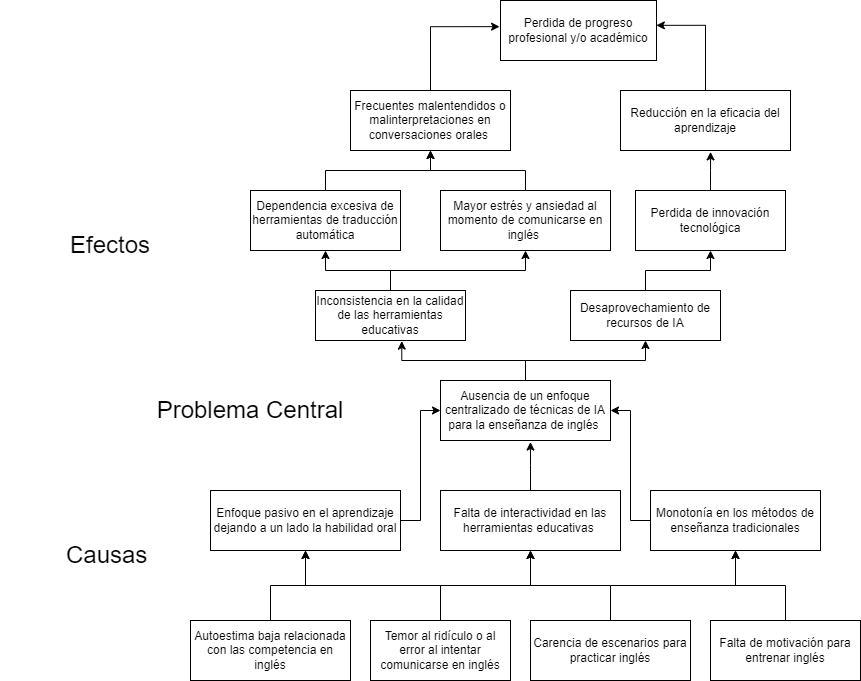
\includegraphics[width=1\linewidth]{Imagenes/seminario Arbol de problemas.png}
    \caption{Árbol de problemas}
    \label{fig:enter-label}
\end{figure}





 
 




\section{Objetivos}

Los objetivos descritos en el siguiente apartado fueron planteados con base en la organización y sistematización de la taxonomía de Bloom.

\subsection{Objetivo General}

Desarrollar un prototipo web para apoyar la enseñanza del idioma inglés, adaptando algoritmos de PLN y técnicas de gamificación.

\subsection{Objetivos Específicos}
\begin{enumerate}
    \item Analizar técnicas de gamificación, Algoritmos de Procesamiento del Lenguaje Natural (PLN), temas de ingles según el Marco Común Europeo de Referencia (MCER) nivel B1 y metodologías de enseñanza, para una experiencia interactiva y adecuada al usuario.
    \item Diseñar los artefactos necesarios para la estructura del prototipo.
    \item Implementar la solución diseñada para el prototipo web.
    \item Evaluar la usabilidad del prototipo, con el fin de que la plataforma sea efectiva y agradable al usuario.

\begin{table}[H]
\begin{tabular*}{\textwidth}{|p{0.05\textwidth}|p{0.4\textwidth}|p{0.5\textwidth}|}
\cline{1-3}
\multicolumn{1}{|c|}{\cellcolor[gray]{0.9} \textbf{No}} & \multicolumn{1}{|c|}{\cellcolor[gray]{0.9} \textbf{Objetivo Específico}} & \multicolumn{1}{|c|}{\cellcolor[gray]{0.9} \textbf{Resultado Esperado}} \\

\cline{1-3}
\textbf{1} & Analizar técnicas de gamificación, Algoritmos de Procesamiento del Lenguaje Natural (PLN), temas de ingles según el Marco Común Europeo de Referencia (MCER) nivel B1 y metodologías de enseñanza, para una experiencia interactiva y adecuada al usuario. & 
\begin{itemize}[left=0pt] 

    \item Informe con las técnicas de gamificación y algoritmos de procesamiento del lenguaje natural seleccionados.
    \item Reporte de las metodologías de enseñanza y temas de inglés escogidos para el prototipo.
\end{itemize} \\

\cline{1-3}
\textbf{2} & Diseñar los artefactos necesarios para la estructura del prototipo.  & 
\begin{itemize}[left=0pt]
    \item Archivo con los mockups de la interfaz del prototipo web.

    \item Esquema de la base de datos.

    \item Diagrama de la arquitectura web para prototipo.

\end{itemize} \\
\cline{1-3}

\textbf{3} & Implementar la solución diseñada para el prototipo web. & 
\begin{itemize}[left=0pt]

    \item Código con la implementacion de los algoritmos de PLN adaptados para su uso y de las técnicas de Gamification.
    
    \item Código fuente del frontend y backend del prototipo web.
\end{itemize} \\
\cline{1-3}
\textbf{4} & Evaluar la usabilidad del prototipo, con el fin de que la plataforma sea efectiva y agradable al usuario. & 
\begin{itemize}[left=0pt] 
    \item Plan de pruebas de evaluación sobre el prototipo.
    \item Reporte con el análisis y conclusiones de las pruebas realizadas.
\end{itemize} \\
\cline{1-3}
\end{tabular*}
\centering
\caption{Resultados esperados}
\end{table}


\newpage
\section{Antecedentes}

\textbf{Elsa Speak: }
La inteligencia artificial se ha convertido en un tema a tratar en la enseñanza de  lenguajes por la razón de que puede asistir y mejorar el aprendizaje de lenguajes para todos los niveles de educación. ELSA Speak es un aplicación de Automatic Speech Recognition (ASR) usada para enseñar pronunciación, estudia cómo los estudiantes escuchan, hablan, vocalizan y aciertan palabras en inglés basado un lenguaje oral. ELSA Speak puede incrementar las habilidades en el idioma inglés de los estudiantes, llegando a motivarlos a continuar su proceso de formación y/o aprendizaje \cite{kholis2021elsa}.
\\
\\
\textbf{Duolingo: }
El mobile learning es un tipo de actividad de aprendizaje que se sirve a través de dispositivos móviles los cuales no requieren que el estudiante esté en una ubicación geográfica en particular, Duolingo es una de las aplicaciones MALL (Mobile-Assisted language learning) más dominantes e influyentes en este campo, siendo una fuerte representación del uso de gamificación para la enseñanza de idiomas, implementando un sistema de retos, recompensas,  un sistema de niveles y de clasificación basados en los logros que obtiene la el estudiante a medida que va aprendiendo un determinado idioma \cite{shortt2023gamification}.
\\
\\
\textbf{ChatGPT: }
El rápido avance de la inteligencia artificial ha brindado soporte a diversos campos incluido el aprendizaje de idiomas, los sistemas de chat basados en IA, como ChatGpt han demostrado su potencial en el desarrollo de habilidades comunicativas en el idioma inglés. Este chat da la oportunidad a los estudiantes de tener interacciones de lenguaje natural en un entorno simulado, esto se da gracias a la implementación de algoritmos de PLN y ML. El uso de este sistema puede mejorar la confianza y la competencia comunicativa de los estudiantes interesados \cite{chicaiza2023aplicaciones}.
\\
\\
\textbf{VIDEOJUEGO PARA EL APOYO A LA ENSEÑANZA DE INGLÉS PARA LOS ESTUDIANTES DE INGENIERÍA DE SISTEMAS DE LA UNIVERSIDAD DEL VALLE SEDE TULUÁ:  }
Trabajo de grado del Ingeniero de Sistemas Luiz Fernando Quintero Castaño, en el cual aborda el apoyo a la enseñanza de inglés en base a un videojuego, utilizando técnicas de gamificación para obtener la “experiencia de juego”, Assessing the core Elements of the Gaming Experience \cite{calvillo2015assessing} juega un papel importante en las técnicas de gamification utilizadas en el proyecto \cite{quintero2018videojuego}.
\\
\\
\textbf{Prototipo de una aplicación de procesamiento de lenguaje natural aplicando traducción a lengua de señas colombiana en dispositivos móviles: }
Trabajo de grado de los Ingenieros de Sistemas Alejando Azcarate Trujillo y Karem Lizeth Torres Ríos ambos Egresados de la Universidad del Valle sede Tuluá, en el cual aborda su proyecto en base al diseño, modelado e implementación de un prototipo de aplicación móvil utilizando llamado Speech To Sings el cual utiliza Modelos Ocultos de Markov  con la finalidad de apoyar el proceso de comunicación entre las personas con discapacidad auditiva \cite{azcarate2020prototipo}.
\\
\\
\textbf{Objetos Virtuales de Aprendizaje con elementos de gamificación para el Apoyo de la Asignatura Fundamentos de Programación del Programa Académico de Ingeniería de Sistemas de la Universidad del Valle Sede Tuluá: }
Trabajo de grado de los Ingenieros de Sistemas Paula Andrea Corre Villalobos y Marisol Davila Escobar ambos Egresado de la Universidad del Valle sede Tuluá, en el cual se busca utilizar Objetos Virtuales de Aprendizaje (OVAs) [16] que contribuyan en la disminución de la deserción de la Asignatura académica Fundamentos de Programación de la Universidad del Valle sede Tuluá. Las técnicas de gamificación utilizadas en el proyecto se basan en la pirámide de los Elementos de Gamificación de Kevin Werbach \cite{correa2018objetos}.

\input{capitulo1/Metodología}
\newpage
\section{Justificación}

El mejoramiento de la comprensión oral en ingles de la población bilingüe en Colombia es un desafió de gran relevancia tanto nivel académico como socioeconómico. El poco dominio de la lengua inglesa contribuye a la perdida de oportunidades laborales y académicas, tal como lo evidencian los puntajes promedio del examen saber 11 (48 para el calendario A y 72 para el calendario B en 2020) pues este examen sirve como prueba de que los jóvenes pre-universitarios no cuentan con un nivel satisfactorio para pasar exámenes de admisión de universidades que estén en este idioma O que tengan una prueba del dominio del mismo, esto trae consigo que el estudiante pierda, en primera instancia, las nuevas oportunidades académicas que se le presentan. Elevar estos resultados aumentaría y posicionaría a los jóvenes colombianos en mejores condiciones competitivas dentro de un mercado laboral globalizado.
\\
\\
Desde el ámbito educativo, es fundamental promover entornos prácticos de inmersión más allá del aula, que permitan incorporar el uso del inglés en la vida diaria y establecer una rutina constante de práctica del idioma, evitando metodologías monótonas y/o ortodoxas que no promueven la asimilación natural de la lengua. Al implementar soluciones tecnológicas activas que faciliten la practica continua (plataformas de interacción oral, videojuegos o comunidades de intercambio cultural) permitirá mantener la motivación y reforzar la apropiación del idioma, evitando el desuso del conocimiento adquirido de este idioma.
\\
\\
El fortalecimiento del ingles contribuye directamente al desarrollo social y económico del país, Las empresas adoptan cada vez mas políticas bilingües con el objetivo de obtener un mayor alcance, ya que el uso del ingles en el ámbito laboral trae consigo negociaciones internacionales y proyectos de investigación en conjunto con otras naciones, lo que resulta en una mayor competitividad en el mercado \cite{cronquist2017aprendizaje}. Un mayor numero de profesionales con competencia oral avanzada impulsaría así la llegada de inversión extranjera, el intercambio cultural y una participación mas activa de Colombia en un mercado global y académico.
\\
\\
Aprovechar las infraestructuras digitales ya existentes (internet, dispositivos móviles, computadores portátiles, tabletas, etc) responde a la necesidad de un aprendizaje flexible (bleend learning).
\\
\\
El desarrollo de este proyecto busca ofrecer una solución innovadora que facilite la practica constante del idioma ingles a través de sistemas que implementen modelos e procesamiento de lenguaje natural. Al implementar una plataforma que estimule la fluidez oral del idioma, se genera oportunidades reales de inmersión lingüística para las personas carentes de espacios adecuados para afianzar sus conocimientos. Esto no solo fortalecerá las competencias comunicativas en ingles de la población bilingüe colombiana, sino que también contribuirá a cerrar brechas académicas, sociales y culturales.



%%%%%%%%%%%%%%%%%%%%%%%%%%%%%%% Capitulo 2 %%%%%%%%%%%%%%%%%%%%%%%%%%%%%%%

\chapter{Alcance del proyecto}
\vspace{-2em}
\section{Declaración del alcance}

El presente proyecto desarrolló de un prototipo web con la finalidad de brindar ayuda al aprendizaje de inglés utilizando PLN y Gamificación para personas que deseen mejorar sus conocimientos de este idioma en Colombia con un nivel de conocimiento base de A2, dentro de un plazo de 8 meses, utilizando un temario según los niveles de inglés descritos según el Marco Común Europeo de Referencia para las lenguas (MCER), basado en un nivel B1 \cite{mcer2002} como guía para su enseñanza. Se implementarán técnicas de procesamiento de lenguaje natural para el desarrollo y funcionamiento del sistema, además contará con mecánicas de gamificación para que los usuarios se apropien del conocimiento de una manera de reto y desarrollen su competitividad con el fin de adquirir y ampliar el uso cotidiano del inglés.
\\
\\
Es necesario recalcar que para el idóneo desarrollo del proyecto se tienen ciertas restricciones y especificaciones que se deben de plantear y tener en cuenta, los cuales son:

\subsection{Supuestos}

\begin{itemize}
    \item Normalidad académica durante el desarrollo del proyecto.
    \item Continuidad del director del trabajo de grado.
    \item No ocurrencia de eventos imprevistos durante la realización del proyecto.
    \item Acceso a la información necesaria para el proyecto, así como la implementación de las tecnologías.
\end{itemize}
\subsection{Restricciones}

\begin{itemize}
    \item El tiempo de desarrollo del proyecto es de ocho (8) meses, los cuales comprenden un total de dos (2) períodos académicos.
    \item El hardware utilizado para el proyecto será el que esté a disposición del estudiante.
    \item Se implementarán un mínimo de tres (3) algoritmos de procesamiento de lenguaje natural.
    \item Se implementarán un mínimo de dos (2) técnicas de gamificación para cumplir el fin del proyecto.
\end{itemize}
\vfill


%%%%%%%%%%%%%%%%%%%%%%%%%%%%%%% Capitulo 3 %%%%%%%%%%%%%%%%%%%%%%%%%%%%%%%

\chapter{Marco referencial}

\section{Marco teórico}

\textbf{La importancia del aprendizaje de idiomas en un mundo globalizado: }Desde el siglo xix el idioma inglés se fue convirtiendo en un idioma obligado para las transacciones comerciales y de toda índole de negocios, tanto en los países desarrollados como en los del tercer mundo,  la globalización ha hecho de este idioma un lenguaje global, y este factor ha llevado a que sea incluido en negocios, cultura, e inclusive dentro de las aulas en países que no tienen este idioma \cite{ibm_pln} como lengua oficial. De este modo surge la necesidad de aprender una lengua extranjera que permita comunicarnos con otros países, y así poder derribar una barrera más entre la cultura y las relaciones internacionales de cada país.
\\
\\
\textbf{Teoría de la conectividad: }Es un modelo de aprendizaje que reconoce el cambio necesario de una sociedad en la que el aprendizaje ya no es una actividad individual, el impacto de las nuevas herramientas tecnológicas para la enseñanza de un lenguaje extranjero proporciona una mejoría en las habilidades de aprendizaje para los estudiantes.\cite{martinez2020herramientas}.
\\
\\
\textbf{El uso de la gamificación para procesos educativos: }La gamificación es la utilización de elementos de diseño de videojuegos en contextos que no son de juego, una técnica en orden de conseguir mejores resultados en el proceso de enseñanza-aprendizaje, posee elementos y técnicas propias de los juegos que se pueden explotar para poder facilitar la interiorización de conocimientos de una forma más divertida y llamativa. Dentro del ámbito del aprendizaje del inglés \cite{molina2021gamificacion}, la gamificación se convierte en una gran oportunidad para mejorar habilidades de expresión oral.
\\
\\
\textbf{Procesamiento de Lenguaje Natural (PLN) en la enseñanza de idiomas: }El procesamiento de lenguaje natural usa distintas reglas gramaticales y lingüísticas como tiempos gramaticales, sistemas semánticos, morfemas etc. Con el fin de desarrollar sistemas de software aplicados a un lenguaje en específico, es un proceso efectivo para asistir a los estudiantes en el proceso de aprendizaje científico, implementando \cite{alhawiti2014natural} PLN en el ámbito educacional no solo ayuda en el desarrollo efectivo del lenguaje, sino también a mejorar el rendimiento académico.Utilizando técnicas de procesamiento de lenguaje Natural se pueden desarrollar estrategias educacionales, que puedan asistir al buen aprendizaje y enseñanza.
\vfill
\subsection{Marco Conceptual}

\textbf{Competencia lingüística: }Habilidad esencial para comunicarse en un idioma, permitiendo la interacción efectiva en diversos contextos. Esta competencia implica no solo el dominio del vocabulario y la gramática, sino también la capacidad de comprender y expresar ideas de manera fluida y precisa \cite{martinez2020herramientas}.
\\
\\
\textbf{Hugginface: }
Hugging Face \cite{Jain2022} es una empresa franco-estadounidense fundada en 2016, reconocida por su contribución al desarrollo de herramientas de código abierto en el ámbito del aprendizaje automático y, en particular, del procesamiento de lenguaje natural (PLN). Su plataforma proporciona una amplia gama de recursos, incluyendo modelos preentrenados, conjuntos de datos y bibliotecas que facilitan la implementación y despliegue de aplicaciones de inteligencia artificial. Entre sus productos más destacados se encuentra la biblioteca Transformers, que ofrece implementaciones de modelos de vanguardia como BERT y GPT, permitiendo a investigadores y desarrolladores acceder y utilizar estas tecnologías de manera eficiente.
\\
\\
\textbf{Procesamiento del lenguaje natural (PLN): } Se refiere a una parte de la inteligencia artificial que se ocupa en dar a las computadoras la capacidad de comprender textos y palabras habladas de la misma manera que los seres humanos, combina la lingüística computacional con modelos estadísticos, con el fin de permitir a las computadoras procesar el lenguaje humano \cite{ibm_pln} en forma de texto, datos o datos de voz, para comprender su significado completo.
\\
\\
\textbf{SQuAD: } (Stanford Question Answering Dataset) es un conjunto de datos de comprensión lectora desarrollado por la Universidad de Stanford. Consiste en preguntas formuladas por trabajadores sobre un conjunto de artículos de Wikipedia, donde la respuesta a cada pregunta es un segmento de texto del pasaje correspondiente. Este conjunto de datos se utiliza ampliamente para entrenar y evaluar sistemas de respuesta a preguntas en el campo del procesamiento de lenguaje natural \cite{Rajpurkar2016}.
\\
\\
\textbf{RACE: } (ReAding Comprehension from Examinations) es un conjunto de datos de comprensión lectora a gran escala, recopilado de exámenes de inglés diseñados para estudiantes de secundaria en China. El conjunto consta de aproximadamente 28,000 pasajes y cerca de 100,000 preguntas generadas por expertos humanos (profesores de inglés), cubriendo una variedad de temas cuidadosamente diseñados para evaluar la capacidad de comprensión y razonamiento de los estudiantes. Ademas la alta proporción de preguntas que requieren razonamiento, lo que lo convierte en un recurso valioso para la investigación y evaluación en comprensión de lectura automática \cite{Lai2017}.
\\
\\
\textbf{Word2Vec: } Word2Vec es una técnica desarrollada por Mikolov et al. en 2013 que utiliza redes neuronales para aprender representaciones vectoriales de palabras a partir de grandes corpus de texto \cite{mikolov2013}.
\\
\\
\textbf{GloVe: } (Global Vectors for Word Representation) es un modelo desarrollado por Pennington et al. en 2014 que combina las ventajas de los modelos basados en conteo global y los modelos predictivos como Word2Vec. Construye una matriz de coocurrencia de palabras a partir de un corpus y aprende representaciones vectoriales que capturan las relaciones de coocurrencia entre palabras \cite{Pennington2014}.
\\
\\
\newpage
\textbf{Transformadores: } Son una arquitectura de red neuronal diseñada para procesar datos secuenciales, como texto o audio, mediante un mecanismo llamado atención. Este mecanismo permite al modelo enfocarse en diferentes partes de la entrada simultáneamente, capturando relaciones contextuales a largo plazo. \cite{vaswani2023attentionneed}.
\\
\\
\textbf{word embeddings:} Son representaciones numéricas de palabras en un espacio vectorial. En lugar de tratar las palabras como entidades aisladas, los word embeddings las representan como vectores de números reales, permitiendo que palabras con significados similares tengan representaciones cercanas en este espacio \cite{wordembeddingssurvey}.

\begin{figure}[h]
  \centering
  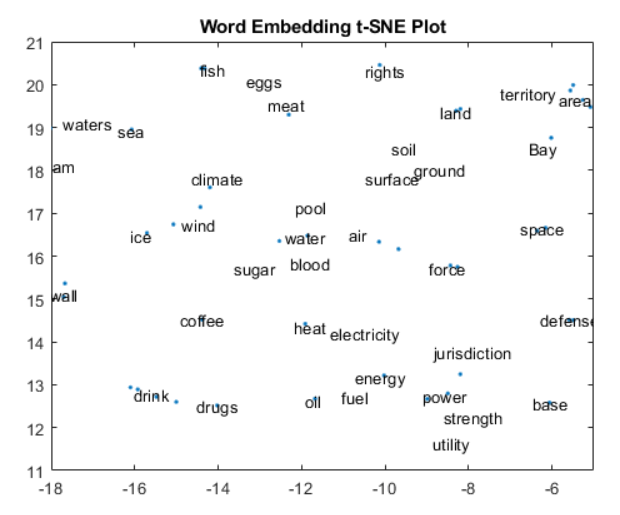
\includegraphics[width=0.5\linewidth]{Imagenes/word emmbedings.png}
  \caption{Representación de Word Emmbedings}
  Fuente: Visualize word embeddings \cite{mathworks1}
  \label{fig:word_emmbedings}
\end{figure}

\newpage
\textbf{GPT: Generative Pre-trained Transformer}

Este modelo utiliza una arquitectura de transformadores centrada exclusivamente en el decodificador unidireccional, lo que le permite generar texto de manera auto regresiva, prediciendo cada palabra basándose únicamente en las palabras anteriores en la secuencia.

\begin{figure}[H]
  \centering
  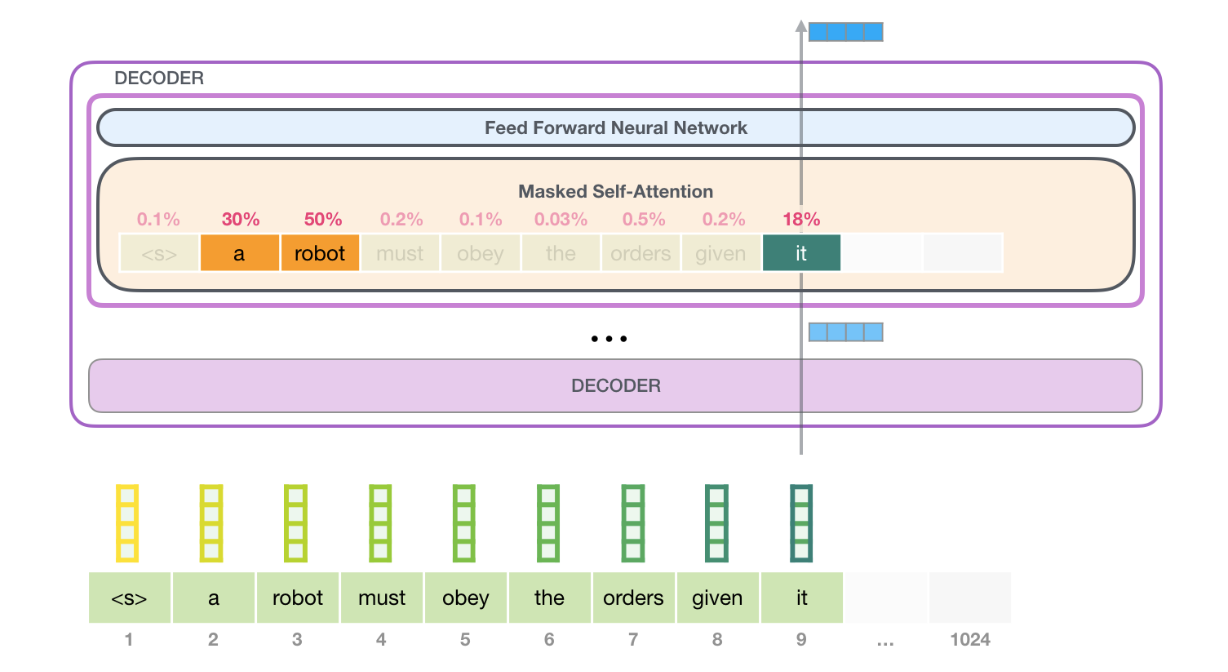
\includegraphics[width=0.8\linewidth]{Imagenes/gpt mascara de atencion.png}
  \caption{Arquitectura de GPT-2.}
  Fuente: The illustrated gpt-2 \cite{alammar2018gpt2}.
  \label{fig:gpt2_flow}
\end{figure}


La Fig.~\ref{fig:gpt2_flow} muestra el flujo interno de GPT-2:
\begin{itemize}
  \item Cada token de entrada (en la parte inferior) se convierte en un embedding posicional y se alimenta al primer bloque \emph{decoder}.
    \item Dentro de cada bloque \emph{Decoder}, la operación de \emph{Masked Self-Attention} evita que el modelo “mire” palabras que aún no han sido generadas. Es decir, cuando GPT-2 está prediciendo el token $t$, esta capa solo le permite revisar la información de los tokens anteriores (1, 2, ..., $t-1$), bloqueando cualquier dato posterior a $t$. De este modo, el modelo aprende a generar cada palabra basándose únicamente en el contexto previo, sin filtrar información del futuro, lo cual garantiza que la predicción sea verdaderamente auto-regresiva.

  \item Después de la atención, una red (barra celeste) refina la representación antes de pasarla al siguiente bloque.
  \item Tras apilar varias capas de este tipo (rectángulos lila), el nivel superior proyecta la salida en logits sobre el vocabulario y escoge la palabra más probable.  
\end{itemize}

\newpage
\textbf{BERT: } (Bidirectional Encoder Representations from Transformers), propuesto por Devlin et al. en 2019, es un modelo basado en transformadores que se pre-entrena en grandes corpus de texto. La bidireccionalidad de BERT permite que cada token considere el contexto completo en ambas direcciones, mejorando la comprensión del lenguaje.

\begin{figure}[H]
  \centering
  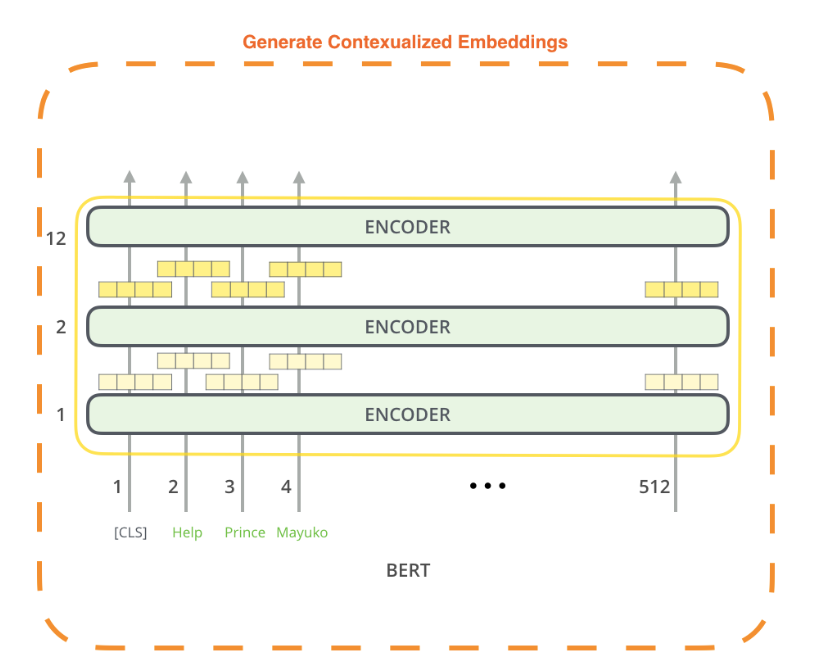
\includegraphics[width=0.8\textwidth]{Imagenes/arquitectura_bert.png}
  \caption{Arquitectura de BERT base}
   Fuente: The illustrated BERT \cite{alammar2018bert}.
  \label{fig:bert_architecture}
\end{figure}

La Fig.~\ref{fig:bert_architecture} muestra el flujo interno de BERT en donde:

\begin{itemize}

    \item BERT toma una secuencia de tokens que incluye un token especial de clasificación \texttt{[CLS]} seguido de tokens como "Help", "Prince", y "Mayuko".

    \item BERT base utiliza 12 capas de encoders (codificadores) para procesar los tokens. Cada capa aplica atención bidireccional, permitiendo que cada token considere el contexto completo de los otros tokens dentro de la secuencia (es decir, tanto antes como después del token a predecir).

    \item A medida que los tokens atraviesan las capas de encoders, se generan representaciones de salida para cada uno. Esto contribuye a la capacidad de BERT para contextualizar palabras y proporcionar representaciones ricas en significado, útiles para diversas tareas de procesamiento de lenguaje natural.

\end{itemize}

\textbf{T5: }(Text-to-Text Transfer Transformer), es un modelo de tipo encoder-decoder basado en la arquitectura Transformer. Su principal innovación es tratar todas las tareas de procesamiento de lenguaje natural (PLN) como problemas de entrada y salida de texto (text-to-text).

\begin{figure}[H]
  \centering
  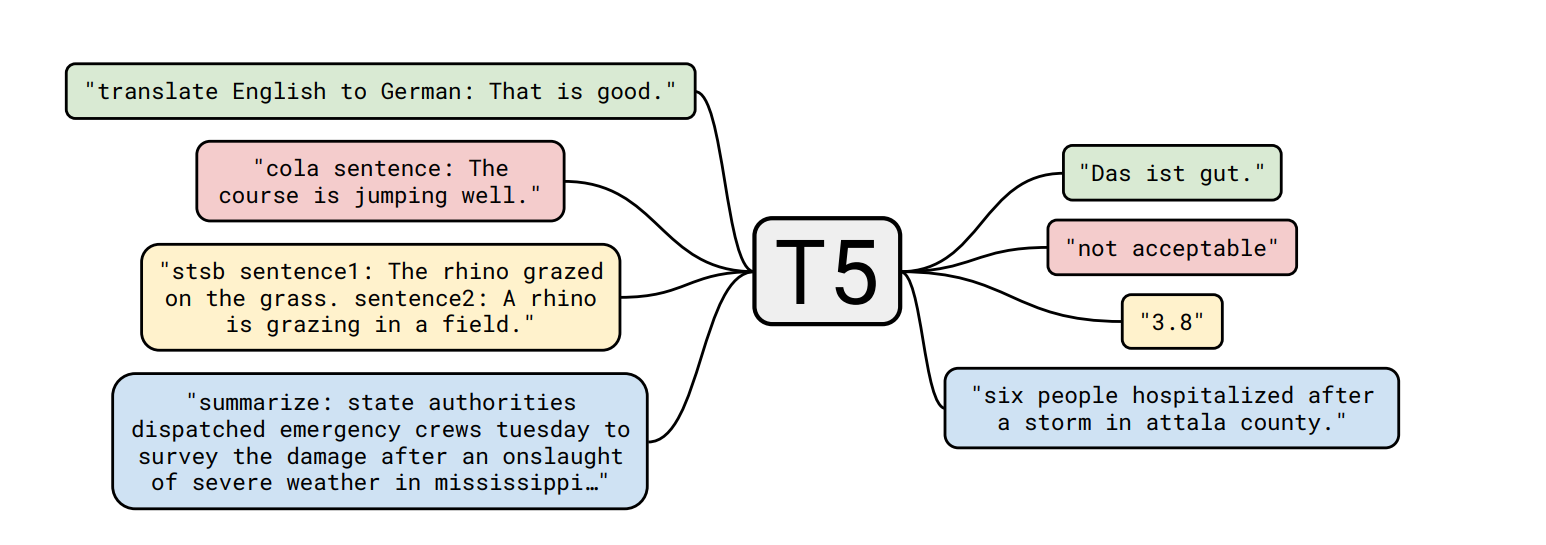
\includegraphics[width=0.7\linewidth]{Imagenes/t5.png}
  \caption{Representación gráfica t5}
  Fuente: Exploring the limits of t5 \cite{transferttt}
  \label{fig:t5_summary}
\end{figure}

\textbf{Inteligencia artificial: } Es un campo que combina la informática y conjuntos de datos robustos para permitir la resolución de problemas, engloba los subcampos del aprendizaje automático y el aprendizaje profundo \cite{ibm_ia} compuestos por algoritmos matemáticos, con el fin de hacer que la computadora “piense” por sí sola, y si realiza predicciones clasificaciones basadas en datos de entrada (preprocesamiento de datos).
\\
\\
\textbf{perplejidad: }
La perplejidad cuantifica la incertidumbre de un modelo al predecir la siguiente palabra en una secuencia. Matemáticamente, se define como la exponencial de la entropía cruzada promedio negativa \cite{huggperplexity}.

\textbf{Gamificación: } El concepto de gamificación consiste en el uso de elementos de juego en contextos no lúdicos. Se basa en el éxito de la industria de los videojuegos, las redes sociales y décadas de investigación en psicología humana, con el fin de aumentar la participación y motivación del usuario en un contexto dado \cite{flores2015using}. Además, la gamificación crea en los usuarios una sensación de compromiso a medida que avanzan en la realización de procesos y la finalización de tareas.
\\
\\
\textbf{Aplicación web: } Es un software que se ejecuta en el navegador web y es accesible desde diferentes dispositivos, ya sean personales o empresariales. Sin embargo, no se descarga en el dispositivo; se ejecuta en un servidor que se comunica a través de internet para, finalmente, llegar al navegador web que está realizando la petición \cite{aws_webapp}.


%%%%%%%%%%%%%%%%%%%%%%%%%%%%%%% Capitulo 4 %%%%%%%%%%%%%%%%%%%%%%%%%%%%%%%

\chapter{Análisis de Fundamentos}
\section{Metodologías de enseñanza}

\subsection{Competencias MCER}

El Marco Común Europeo de Referencia (MCER) es un estándar internacional que proporciona una base común para diseñar programas de lenguas, exámenes y materiales didácticos. Este marco define lo que los estudiantes deben aprender para comunicarse eficazmente en una lengua extranjera, incluyendo las competencias en las distintas destrezas lingüísticas, así como los conocimientos del idioma y la comprensión cultural. El MCER establece seis niveles de dominio (A1, A2, B1, B2, C1 y C2) que permiten medir el progreso del estudiante de forma objetiva.
\\
\\
Dado que el alcance de este proyecto está dirigido a personas en Colombia que deseen mejorar sus conocimientos del idioma inglés y que poseen un nivel de competencia entre A2 y B1, es importante especificar los descriptores de estos niveles. Para ello, tomamos como referencia la guía oficial del Consejo de Europa y el Instituto Cervantes \cite{mcer2002}.

\begin{table}[H]
\centering
\small
\begin{tabular}{|p{4cm}|p{10cm}|}
\hline
\textbf{Nivel} & \textbf{Descripción  escala global} \\
\hline
\textbf{A2 (Usuario básico)} & Es capaz de comprender frases y expresiones de uso frecuente relacionadas con áreas de experiencia que le son especialmente relevantes (información básica sobre sí mismo y su familia, compras, lugares de interés, ocupaciones, etc.). Sabe comunicarse a la hora de llevar a cabo tareas simples y cotidianas que no requieran más que intercambios sencillos y directos de información sobre cuestiones que le son conocidas o habituales. Sabe describir en términos sencillos aspectos de su pasado y su entorno, así como cuestiones relacionadas con sus necesidades inmediatas. \\
\hline
\textbf{B1 (Usuario independiente)} & Es capaz de comprender los puntos principales de textos claros y en lengua estándar si tratan sobre cuestiones que le son conocidas, ya sea en situaciones de trabajo, de estudio o de ocio. Sabe desenvolverse en la mayor parte de las situaciones que pueden surgir durante un viaje por zonas donde se utiliza la lengua. Es capaz de producir textos sencillos y coherentes sobre temas que le son familiares o en los que tiene un interés personal. Puede describir experiencias, acontecimientos, deseos y aspiraciones, así como justificar brevemente sus opiniones o explicar sus planes. \\
\hline
\end{tabular}
\caption{Descriptores generales de los niveles A2 y B1 del MCER}
Fuente: Consejo de Europa MCER \cite{mcer2002}
\label{tab:descriptores-mcer}
\end{table}

\subsection{Temas de ingles}

\section*{Introducción}

En esta sección se presenta una recopilación de temas gramaticales específicos correspondientes a los niveles A2 (pre-intermedio) \cite{britisha1a2grammar} y B1 (intermedio) \cite{britishb1b2grammar} del MCER, basándose en los recursos proporcionados por el British Council. Estos temas son fundamentales para identificar y justificar el nivel de competencia.

\section*{Nivel A2 – Usuario Básico (Pre-intermedio)}

Según el British Council \cite{britisha1a2grammar}, los estudiantes en el nivel A2 deben ser capaces de comprender y utilizar estructuras gramaticales básicas en contextos cotidianos. Algunos de los temas que están en este nivel son:

\begin{itemize}[leftmargin=*, label=--]
    \item \textbf{Artículos:} uso de \textit{a}, \textit{an}, \textit{the} y casos donde no se utiliza artículo.
    \item \textbf{Adjetivos terminados en \textit{-ed} y \textit{-ing}:} diferencias entre \textit{bored} y \textit{boring}.
    \item \textbf{Adverbios de frecuencia:} \textit{always}, \textit{usually}, \textit{sometimes}, \textit{never}.
    \item \textbf{Comparativos y superlativos:} \textit{older}, \textit{the oldest}, \textit{more interesting}, \textit{the most interesting}.
    \item \textbf{Pronombres:} personales, posesivos, demostrativos y reflexivos.
    \item \textbf{Tiempos verbales:} presente simple, pasado simple, futuro con \textit{will} y \textit{going to}.
\end{itemize}

\section*{Nivel B1 – Usuario Independiente (Intermedio)}

En el nivel B1 \cite{britishb1b2grammar}los estudiantes deben ser capaces de comprender y utilizar estructuras gramaticales complejas en una variedad de contextos. Algunos de los temas que están en este nivel son:

\begin{itemize}[leftmargin=*, label=--]
    \item \textbf{Adjetivos gradables y no gradables:} uso de intensificadores como \textit{a bit}, \textit{really}, \textit{absolutely}.
    \item \textbf{Uso de mayúsculas y apóstrofes:} reglas de puntuación y ortografía.
    \item \textbf{Tiempos verbales:} presente perfecto, pasado perfecto, futuro continuo, pasado continuo.
    \item \textbf{Voz pasiva:} formación y uso en diferentes tiempos verbales.
    \item \textbf{Condicionales:} segundo y tercer condicional para situaciones hipotéticas.
    \item \textbf{Verbos frasales (phrasal verbs):} uso y significado en contextos variados.
\end{itemize}

\section*{Relevancia de los temas en el prototipo}

La identificación y comprensión de estos temas gramaticales son esenciales para evaluar y justificar el nivel de competencia lingüística en inglés. Utilizando los recursos proporcionados por el British Council \cite{britishcouncilgrammar}, se puede asegurar una base sólida y confiable para el aprendizaje y la enseñanza del idioma.

Si bien se han identificado y categorizado los temas gramaticales más relevantes de los niveles A2 y B1, es importante destacar que su incorporación en el prototipo no obedece a fines explicativos o pedagógicos aislados. Dado que el prototipo está diseñado para generar textos, preguntas y respuestas, la selección de estos contenidos tiene como propósito principal profundizar en el perfil de la población objetivo, es decir, a la población bilingüe Colombiana cuyo nivel de inglés se sitúa entre A2 y B1.

Además, los temas identificados sirven como base para justificar lingüísticamente la validez de los textos generados por el prototipo. Esta justificación se respalda mediante la encuesta de niveles de inglés (capítulo 7), la cual fue aplicada con el fin de evaluar la adecuación del contenido lingüístico incluido en las lecciones. Dicha encuesta fue dirigida exclusivamente a docentes con experiencia en la enseñanza del inglés, lo que garantiza un respaldo experto en la validación del nivel y calidad del contenido generado.

\subsection{Metodolog\'ias actuales}
La enseñanza del inglés como lengua extranjera ha evolucionado a lo largo del tiempo, adoptando diversos enfoques y metodologías que van desde modelos tradicionales hasta propuestas más centradas en la comunicación y en el estudiante. Entre las metodologías más empleadas se encuentran el método gramatical-traductivo, \cite{metodogramaticatrad}, basado en el análisis detallado de las reglas gramaticales y sus excepciones, aplicándose a través de la traducción de oraciones y textos; el enfoque comunicativo, \cite{enfoquecomunicativo}, que promueve el uso de textos, grabaciones y actividades que reproducen situaciones reales fuera del aula; el aprendizaje basado en tareas (TBLT), \cite{TBLT}, que se centra en la realización de tareas significativas en la lengua meta para fomentar la comunicación efectiva; y el aprendizaje blended (Blended Learning) \cite{salinas2010entrenamiento}, que integra la instrucción presencial con el uso de recursos digitales para enriquecer el proceso educativo.
\\
\\
Estas metodolog\'ias han contribuido significativamente al desarrollo de competencias ling\"u\'isticas; sin embargo, presentan ciertos desaf\'ios. Muchas veces, los enfoques tradicionales resultan mon\'otonos, poco motivadores y desconectados de los intereses y contextos reales de los estudiantes. Incluso las propuestas m\'as modernas pueden verse limitadas si no logran captar la atenci\'on del aprendiz o si no fomentan su participaci\'on activa y constante.
\\
\\
Ante estas limitaciones, ha emergido con fuerza la gamificaci\'on como una estrategia pedag\'ogica innovadora que transforma el aprendizaje del ingl\'es en una experiencia l\'udica, interactiva y motivadora. La gamificaci\'on se basa en incorporar elementos propios del juego (puntos, niveles, recompensas, retos, etc.) en contextos educativos, con el fin de aumentar el compromiso, la autonom\'ia y la motivaci\'on del estudiante.
\\
\\
En este punto también es necesario aclarar la diferencia entre aprender un lenguaje como lengua materna y aprender un lenguaje de forma extranjera (segundo idioma), pues implica procesos distintos \cite{flores2015using}. Mientras que la primera se adquiere de manera natural y espont\'anea en entornos ricos en lenguaje, desde una edad temprana y sin instrucci\'on formal, el aprendizaje de una lengua extrangera, gneralmente ocurre en contextos m\'as restringidos, como el aula, y requiere esfuerzos conscientes y concientes. Esta diferencia impacta directamente en las metodologías empleadas, y resalta la necesidad de estrategias más efectivas, como el blend learning más gamificación, que puedan simular ambientes inmersivos y motivadores similares a los del aprendizaje de la lengua materna.
\\
\\
Considerando los desafíos en la enseñanza del inglés como lengua extranjera, se utilizo para el proyecto el aprendizaje blended con técnicas de gamificación. Esta combinación permite integrar la flexibilidad de los recursos digitales con la interacción presencial, al mismo tiempo que aprovecha el potencial motivador de los elementos lúdicos para fomentar un aprendizaje significativo, contextualizado y motivando al estudiante. Como se observa en la \autoref{tab:descriptores-mcer}, las personas que se encuentran en los niveles A2 y B1 del MCER presentan necesidades específicas en cuanto al desarrollo de sus competencias comunicativas. Por ello, dichas características metodológicas resultan especialmente valiosas para fortalecer las competencias en el contexto colombiano, proporcionando un entorno educativo que favorece el avance progresivo en el dominio del idioma.



\section{Técnicas de gamificación aplicables}

La gamificación ofrece una amplia gama de técnicas que pueden ser aplicadas en contextos educativos para fomentar la motivación, el compromiso y el aprendizaje significativo. Estas estrategias, inspiradas en el diseño de videojuegos, permiten transformar la experiencia educativa en una dinámica más interactiva y centrada en el estudiante. A continuación, se describen algunos de los elementos que más se utilizan para el LESL (Learning English as a Second Language) según una revisión sistemática de elementos de gamificación \cite{Dehghanzadeh2021}, la cual cuenta con el análisis de 96 artículos los cuales fueron filtrados de la siguiente manera para obtener 22  artículos que utilizan técnicas de gamificación para el LESL:

\newpage
\begin{itemize}
  \item Publicaciones que solo utilizan la gamificación era para LESL.
  \item Solo estudios en entornos digitales.
  \item Exclusión de investigaciones centradas en otros idiomas distintos al inglés.
\end{itemize}

\begin{table}[H]
\centering
\begin{tabular}{|l|p{10cm}|}
\hline
\textbf{Elemento de gamificación} & \textbf{Descripci\'on} \\ \hline
Retroalimentaci\'on (Feedback) & Informaci\'on inmediata sobre el desempe\~no del usuario. \\ \hline
Desaf\'io (Challenge) & Retos que ponen a prueba las habilidades del usuario. \\ \hline
Recompensa (Reward) & Beneficios otorgados por completar actividades. \\ \hline
Tabla de clasificaci\'on (Leaderboard) & Lista que muestra el rendimiento comparativo entre los usuarios. \\ \hline
Presi\'on de tiempo (Time pressure) & L\'imite temporal para completar una tarea. \\ \hline
Barra de progreso (Progress bar) & Indicador visual del avance en el aprendizaje. \\ \hline
Puntos (Point) & Unidad num\'erica que cuantifica logros. \\ \hline
Nivel (Level) & Etapa alcanzada seg\'un la acumulaci\'on de logros. \\ \hline
Insignia (Badge) & Distintivo visual que simboliza un logro. \\ \hline
Sistema de puntuaci\'on (Score system) & M\'etodo para calcular el desempe\~no total del estudiante. \\ \hline
Avatar & Representaci\'on gr\'afica del estudiante en el entorno digital. \\ \hline
Historia (Story) & Contexto narrativo que enmarca las actividades. \\ \hline
Narraci\'on (Narration) & Descripci\'on guiada de eventos dentro de la experiencia. \\ \hline
\end{tabular}
\caption{Técnicas comunes de gamificación y sus descripciones breves}
Fuente: Using gamification
to support LESL \cite{Dehghanzadeh2021}.
\end{table}


\subsection{Elementos de gamificación seleccionados}

Para el desarrollo del presente proyecto, el cual esta orientado al aprendizaje del inglés como lengua extranjera, se seleccionaron una combinación de técnicas gamificadas que se ajustan de manera adecuada al objetivo y funciones del prototipo.

\begin{itemize}
\item \textbf{Puntos de experiencia (XP): } como método para cuantificar el progreso tras cada lección completada.
\item \textbf{Insignias: } en función de la acumulación de XP, actuando como incentivo visual y simbólico.
\item \textbf{Días de racha: } para premiar la participación continua y fomentar la constancia en el aprendizaje.
\item \textbf{Ranking de jugadores: } que permite a los usuarios comparar su rendimiento y sentirse parte activa de una comunidad de aprendizaje.
\end{itemize}





\newpage
\section{Panorama de avances en PLN}

Antes de la adopción generalizada de modelos de aprendizaje profundo (Deep Learning Models), el procesamiento de lenguaje natural se basaba en técnicas como la codificación one-hot, que asignaba a cada palabra un vector binario de alta dimensión con un único valor de uno y ceros en las demás posiciones. Sin embargo, este enfoque no capturaba relaciones semánticas entre palabras y resultaba ineficiente para tareas complejas de PLN.
\\
\\
El Procesamiento de Lenguaje Natural ha experimentado avances significativos en la última década, impulsado por el desarrollo de modelos de aprendizaje profundo (Deep Learning). Estos avances han transformado la forma en que las máquinas comprenden y generan lenguaje humano, permitiendo la creación de aplicaciones orientadas a brindar apoyo en distintas áreas. Se han desarrollado herramientas que facilitan la traducción automática, los asistentes virtuales, el análisis de sentimientos, la corrección gramatical, la clasificación de textos, entre muchas otras. Estas aplicaciones han mejorado la eficiencia y accesibilidad en sectores como la educación, la salud, el comercio, la atención al cliente y la investigación científica.
\\
\\
El desarrollo de representaciones distribuidas de palabras, también conocidas como word embeddings, permitió representar palabras como vectores densos en un espacio continuo de menor dimensión. Estas representaciones capturan similitudes semánticas y sintácticas entre palabras, facilitando tareas como la clasificación de texto, la traducción automática y la respuesta a preguntas.
\\
\\
Hoy en dia se tienen diferentes formas de aplicar algoritmos y/o modelos de PLN, como lo son Word2Vec, GloVe, Transformadores, GPT, BERT, RoBERTa etc... A lo que nos planteamos ¿que arquitectura y modelos podemos utilizar para el desarrollo del prototipo?

\section{Búsqueda de modelos}

Es importante utilizar los modelos state-of-the-art disponibles actualmente para evitar las limitaciones de tecnologías anteriores. La arquitectura más reciente, los transformadores, incorpora un mecanismo de auto-atención que resuelve muchos de los problemas presentes en otras arquitecturas de redes neuronales. Por ejemplo, las RNN (Recurrent Neural Network) tienen dificultades para mantener el contexto en textos extensos, mientras que los transformadores, gracias a su mecanismo de atención, manejan eficazmente grandes cantidades de texto. Por ende la mejor opción es utilizar un modelo basado en la arquitectura de redes neuronales de transformadores.
\\
\\
En hugginface podemos encontrar múltiples modelos de aprendizaje automático y aprendizaje profundo, de las cuales se tiene un apartado exclusivamente para modelos enfocados al procesamiento de lenguaje natural, esto nos facilita la búsqueda al poder centralizarla en esta amplia biblioteca de modelos libres creados por su comunidad y empresas como Google, nvidia y deepseek, que suben sus modelos de forma gratuita, para uso libre.

\newpage
\subsection{Generador de texto}

Para el generador de texto en este proyecto, se evaluaron varias versiones del modelo GPT-2 de OpenAI, disponibles en Hugging Face. Se consideraron factores como el tamaño del modelo,la cantidad de parámetros y el valor de la métrica \cite{huggingfacegpt2}.

\begin{table}[H]
\centering
\begin{tabular}{lccc}
\hline
\textbf{Versión} & \textbf{Parámetros (M)} & \textbf{Tamaño Aproximado} & \textbf{Perplejidad en WikiText-2} \\
\hline
GPT-2 Small  & 124  & $\sim$548 MB & 29.41 \\
GPT-2 Medium & 355  & $\sim$1.52 GB & 22.76 \\
GPT-2 Large  & 774  & $\sim$3.25 GB & 19.93 \\
GPT-2 XL     & 1558 & $\sim$6.43 GB & 18.34 \\
\hline
\end{tabular}
\caption{Comparativa de versiones de GPT-2 con perplejidad en WikiText-2.}
Fuente: Metricas de los modelos gpt2 en Hugginface \cite{huggingfacegpt2}.
\end{table}

WikiText-2 es un conjunto de datos muy utilizado en el campo del procesamiento de lenguaje natural para entrenar y evaluar modelos de procesamiento de lenguaje natural el cual, comúnmente es evaluado con una métrica clave para evaluar los modelos entrenados este conjunto de datos, la perplejidad \cite{huggperplexity}. La perplejidad indica qué tan bien un modelo se ajusta a un conjunto de datos; a menor perplejidad, mejor es la capacidad del modelo para predecir el texto.
\\
\\
Aunque los modelos más grandes de GPT-2 (Medium, Large y XL) ofrecen mejoras en ciertas métricas, estas mejoras no siempre son proporcionales al aumento significativo en tamaño y requerimientos computacionales (los pesos son proporcionados vía Hugging Face). Por ejemplo, GPT-2 Small tiene un tamaño de aproximadamente 548 MB, mientras que GPT-2 Medium y GPT-2 Large requieren 1.52 GB y 3.25 GB respectivamente.
\\
\\
En términos de rendimiento, GPT-2 Small logra una perplejidad de aproximadamente 29.41 en el conjunto de datos WikiText-2, lo que indica una capacidad razonable para modelar el lenguaje. Aunque los modelos más grandes pueden mejorar esta métrica, el incremento de la calidad de la generación de texto no justifica el aumento en recursos necesarios para su correcta implementación, especialmente en entornos con limitaciones de hardware, como es el caso en este proyecto.


\subsection{Generadores de pregunta y respuestas}

En el contexto de este proyecto, se optó por utilizar los modelos de Potsawee Manakul \cite{manakul2023} doctor en Ingeniería por la Universidad de Cambridge, especializado en Procesamiento de Lenguaje Natural (NLP), debido a su capacidad para generar tanto preguntas como respuestas a partir de un único modelo, lo que permite una implementación más eficiente al evitar la necesidad de modelos separados para cada tarea, lo cual gana ante los demás modelos de generación de preguntas y respuestas presentes en hugginface.

\subsubsection {Modelo entrenado con SQuAD} Este modelo es el t5-large-generation-race-QuestionAnswer, el cual genera preguntas y respuestas de tipo extractivo, es decir, las respuestas se encuentran directamente en el texto de entrada \cite{potsaweesquad}. es decir solo referirse en donde lo puede encontrar, esto para todo de anexos.

\subsubsection {Modelo entrenado con RACE} El t5-large-generation-squad-QuestionAnswer produce preguntas y respuestas de tipo abstractivo, donde las respuestas pueden ser re-formulaciones o inferencias basadas en el texto de entrada \cite{potsaweerace}.

\subsubsection {Modelo de preguntas incorrectas}
El modelo de generación de respuestas incorrectas es el t5-large-generation-race-Distractor, el cual se integra al sistema de generación de preguntas y respuestas para ambos modelos. Su propósito es generar opciones de respuesta incorrectas que sean plausibles y coherentes con el contexto, lo que enriquece la experiencia de aprendizaje al fomentar una evaluación más efectiva de la comprensión del usuario \cite{potsaweedistractor}.
\\
\\
La elección de optar por el uso de dos modelos especializados (uno entrenado con SQuAD para preguntas extractivas y otro con RACE para preguntas abstractivas) responde a una estrategia orientada a ofrecer al usuario del prototipo dos tipos de preguntas: extractivas y abstractivas. Esta dualidad permite enriquecer la experiencia de aprendizaje al presentar tanto preguntas cuyas respuestas están directamente en el texto como aquellas que requieren inferencia o re-formulación ademas, esta elección optimiza tanto el uso de recursos computacionales como el flujo de trabajo en la implementación del sistema.


\subsection{Modelo de comparación de oraciones}

Para evaluar la precisión de las respuestas proporcionadas por los usuarios en las lecciones, donde se presentan dos opciones, correcta e incorrecta, se implementó el modelo cross-encoder/stsb-roberta-base. Este modelo, basado en la arquitectura RoBERTa, fue entrenado en el conjunto de datos STS Benchmark para predecir la similitud semántica entre pares de oraciones, asignando puntuaciones entre 0 y 1. \cite{stsbrobertabase} Su elección se fundamenta en su alto rendimiento en tareas de similitud textual. Además, al procesar simultáneamente los pares de oraciones, el modelo captura de manera más precisa las relaciones semánticas entre la respuesta del usuario y la respuesta correcta generada por el sistema, facilitando una evaluación efectiva.

\newpage
\section{Elementos seleccionados}

A continuación se sintetizan los componentes y enfoques finalmente adoptados en cada una de las etapas de este capitulo:

\begin{itemize}
  \item \textbf{Temas de ingles según MCER}:
    \section*{Nivel A2}  
        \begin{itemize}
            \item Artículos.
            \item Adjetivos.
            \item Adverbios de frecuencia.
            \item Comparativos y superlativos.
            \item Pronombres.
            \item Tiempos verbales.
        \end{itemize}


    \section*{Nivel B1}
    
    \begin{itemize}
        \item Adjetivos gradables y no gradables.
        \item Uso de mayúsculas y apóstrofes.
        \item Tiempos verbales.
        \item Voz pasiva.
        \item Condicionales.
        \item verbos frasales (phrasal verbs).
    \end{itemize}

  \item \textbf{Enfoque metodológico}:  
    \begin{itemize}
      \item Metodología bleended learning combinado con técnicas de gamificación.
    \end{itemize}

  \item \textbf{Técnicas de gamificación seleccionadas}:  
    \begin{itemize}
      \item Puntos de experiencia (XP).  
      \item Insignias.  
      \item Días de racha (streak).  
      \item Ranking de jugadores.
    \end{itemize}

  \item \textbf{Modelos de PLN preseleccionados}:  
    \begin{itemize}
      \item Generación de texto: \texttt{GPT-2 Small}.  
      \item Preguntas y respuestas:  
        \begin{itemize}
          \item Modelo extractivo: \texttt{t5-large-generation-race-QuestionAnswer}
          \item Modelo abstractivo: \texttt{t5-large-generation-squad-QuestionAnswer}
          \item Generador de respuestas incorrectas: \texttt{t5-large-generation-race-Distractor}
        \end{itemize}
      \item Evaluación de similitud de oraciones: \texttt{cross-encoder/stsb-roberta-base}.
    \end{itemize}
\end{itemize}



%%%%%%%%%%%%%%%%%%%%%%%%%%%%%%% Capitulo 5 %%%%%%%%%%%%%%%%%%%%%%%%%%%%%%%

\chapter{Diseño de artefactos}
\section{Arquitectura del sistema}

\subsection{Tecnologías seleccionadas}
\noindent Hoy en d\'ia, el ecosistema de herramientas y marcos de trabajo para el desarrollo web es muy amplio, abarcando desde bibliotecas para la interfaz de usuario hasta soluciones para el backend y la gesti\'on de tareas en segundo plano. A continuación se tienen diferentes tablas con algunas de las tecnologías mas destacadas para cada uno de los componentes que comprende la arquitectura el prototipo web.

\begin{table}[H]
\centering
\begin{tabular}{|l|p{10cm}|}
\hline
\textbf{Tecnología Frontend} & \textbf{Descripción} \\
\hline
Vue.js & Simplicidad y facilidad de integración, ideal para proyectos ligeros y rápidos de desarrollar. \\
\hline
Angular & Respaldado por Google, con una arquitectura robusta pensada para aplicaciones empresariales de gran escala. \\
\hline
Svelte & Enfoque innovador al compilar sus componentes en JavaScript puro, eliminando el uso del DOM virtual y logrando un mejor rendimiento. \\
\hline
React & Gran versatilidad, integración natural con TypeScript y Tailwind CSS. Arquitectura basada en componentes re-utilizables y escalables. \\
\hline
\end{tabular}
\caption{Tecnologías destacadas para el desarrollo frontend}
\end{table}

\noindent Con base en estas características, se seleccionó React como la tecnología más conveniente y eficiente para el desarrollo de la interfaz de usuario del prototipo.
\\
\\

\begin{table}[H]
\centering
\begin{tabular}{|l|p{10cm}|}
\hline
\textbf{Tecnología API Backend} & \textbf{Descripción} \\
\hline
Django & Conocido por su robustez, seguridad y rapidez de desarrollo. \\
\hline
Flask & Ideal para aplicaciones más pequeñas o que requieren mayor flexibilidad. \\
\hline
Node.js & Basado en JavaScript, permite usar un mismo lenguaje tanto en el frontend como en el backend, promoviendo la uniformidad en el desarrollo. \\
\hline
FastAPI & Ligero y eficiente. Utiliza tipado estático para mejorar la claridad y documentación de las APIs, facilitando la integración con servicios externos.\\
\hline
\end{tabular}
\caption{Tecnologías destacadas para el desarrollo backend}
\end{table}

\noindent Por su eficiencia, facilidad de uso y moderna arquitectura, FastAPI fue seleccionada como la opción ideal para el desarrollo del backend del prototipo.
\\
\\
En el desarrollo de aplicaciones web modernas, contar con un sistema para la gestión de tareas en segundo plano resulta  beneficioso, especialmente cuando se ejecutan procesos intensivos como aquellos relacionados con modelos de inteligencia artificial. Este tipo de soluciones permite liberar al servidor principal de operaciones pesadas, lo cual evita bloqueos o lentitud en la atención de las solicitudes y garantiza una experiencia de usuario más fluida y eficiente. En el caso del presente proyecto, esta necesidad se vuelve aún más relevante al momento de generar lecciones que requieren procesamiento con modelos de IA, lo cual podría afectar negativamente el rendimiento general del sistema. 
\begin{table}[H]
\centering
\begin{tabular}{|l|p{10cm}|}
\hline
\textbf{Tecnología } & \textbf{Descripción} \\
\hline
RQ & Herramienta sencilla para gestionar tareas en segundo plano utilizando Redis como sistema de cola. \\
\hline
Dramatiq & Sistema de colas basado en Python, conocido por su buen rendimiento y facilidad de uso. \\
\hline
Celery & Herramienta madura, compatible con distintos brokers de mensajes y altamente configurable. Se pueden programar tareas periódicas (Celery Beat). \\
\hline
\end{tabular}
\caption{Tecnologías destacadas para la gestión de tareas en segundo plano}

\end{table}

\noindent Dado el contexto del proyecto y la necesidad de procesar tareas intensivas como la generación de lecciones con modelos de IA, se eligió Celery junto con Celery Beat por su robustez y flexibilidad.
\\
\\
En lo que respecta a la gestión de bases de datos dentro del desarrollo del prototipo, se optó por utilizar PostgreSQL y Redis. Esta elección se basa principalmente en la familiaridad previa con estas herramientas, así como en el hecho de que la lógica de integración y manipulación de datos no difiere significativamente entre tecnologías similares, lo que permite enfocar los esfuerzos en otros aspectos más críticos del sistema.

\begin{table}[H]
\centering
\begin{tabular}{|p{3cm}|p{9cm}|}
\hline
\textbf{Tecnología} & \textbf{Descripción} \\
\hline
PostgreSQL & Sistema de gestión de bases de datos relacional, conocido por su estabilidad, conformidad con estándares SQL y capacidades avanzadas como el manejo de tipos de datos complejos y extensiones. \\
\hline
Redis & Almacén de datos en memoria, basado en estructuras clave-valor, ideal para operaciones rápidas y uso como sistema de caché o base de datos secundaria para tareas de alta concurrencia. \\
\hline
\end{tabular}
\caption{Tecnologías utilizadas para la gestión de bases de datos}
\end{table}


Teniendo en cuenta lo anterior se presentan las tecnologías seleccionadas para cada componente de la arquitectura.


\begin{itemize}
    \item \textbf{Frontend:} Implementado con React, TypeScript y Tailwind CSS. Este componente se encarga de la interfaz de usuario, permitiendo la interacci\'on del usuario con las lecciones, preguntas y resultados.
    
    \item \textbf{Backend (API):} Utiliza FastAPI para gestionar las peticiones provenientes del frontend. Este servidor maneja la autenticación, el enrutamiento y la comunicación con la base de datos, así como con los servicios asíncronos. Internamente, sigue una arquitectura basada en el patrón Modelo-Vista-Controlador (MVC).
    
    \item \textbf{Gestión de tareas (as\'incrono):} Se apoya en Celery y Celery Beat para procesar tareas de forma peri\'odica. Este servicio trabaja de forma desacoplada del servidor principal, permitiendo la escalabilidad del sistema.

    \item \textbf{Base de datos NoSQL:} Redis sirve como sistema de almacenamiento en memoria para consultas r\'apidas, evitando el acceso constante a la base de datos. Ademas, Redis se utiliza como el brocker y backend para la cola de tareas en celery, siendo en el index 0 broker y en el indice 1 backend (es decir, donde guarda los estados de las tareas y sus resultados).

    \item \textbf{Base de datos SQL:} Se utiliza PostgreSQL alojado en NeonDB. Esta base de datos almacena toda la informaci\'on relevante del sistema, incluyendo usuarios, rachas, lecciones y preguntas incorrectas.
\end{itemize}

\noindent Esta arquitectura permite una separaci\'on clara de responsabilidades, facilita la escalabilidad del sistema distribuye las cargas entre procesos sincr\'onos y as\'incronos.



\newpage
\section{Explicación del prototipo.}

Antes de profundizar en los detalles del funcionamiento del prototipo, es fundamental presentar su estructura lógica general.
\\
\\
El prototipo está centrado exclusivamente en la entidad usuario, quien es el único actor que interactúa directamente con el sistema. Una vez que accede a la plataforma, el usuario puede visualizar y participar en diversas lecciones, las cuales están compuestas por un conjunto de preguntas.
\\
\\
Cada lección se organiza de forma estructurada, incluyendo un texto base que introduce el tema de la lección, seguido de dos preguntas. Cada pregunta está acompañada por su respuesta correcta y una incorrecta, lo cual permite evaluar la comprensión del usuario.

\section{Diseño de base de datos}
\noindent La base de datos relacional para el prototipo tiene como objetivo central gestionar la información relacionada con los usuarios y su proceso de aprendizaje a través de lecciones y preguntas (dicho proceso se explica a mas detalle en el capitulo 6). Para ello, se estructura en seis (6) tablas principales: \textbf{usuarios}, \textbf{lecciones}, \textbf{preguntas}, \textbf{registro\_preguntas}, \textbf{lecciones\_resueltas} y \textbf{rachas}. Cada una de estas tablas cumple una función específica dentro del sistema y se encuentra relacionada para facilitar el acceso eficiente y coherente a los datos.
\\
\\
A continuación se presenta una descripción breve de cada tabla:
\begin{itemize}
  \item \textbf{usuarios}: almacena la información principal de cada usuario del sistema.
  \item \textbf{lecciones}: contiene los registros de las lecciones generadas, incluyendo su contenido.
  \item \textbf{preguntas}: guarda el contenido de las preguntas asociadas a cada lección.
  \item \textbf{registro\_preguntas}: almacena el resultado de las preguntas que el usuario ha respondido, permitiendo realizar un seguimiento de las preguntas respondidas incorrectamente para reutilizarlas en la sección de preguntas incorrectas del prototipo.
  \item \textbf{lecciones\_resueltas}: registra todas las lecciones que el usuario ya ha completado.
  \item \textbf{rachas}: controla elementos de gamificación, como la cantidad de días consecutivos en los que un usuario ha respondido correctamente al menos una pregunta y la experiencia global obtenida.
\end{itemize}

\subsection{Modelo Entidad Relación }

\begin{figure}[H]
  \centering
  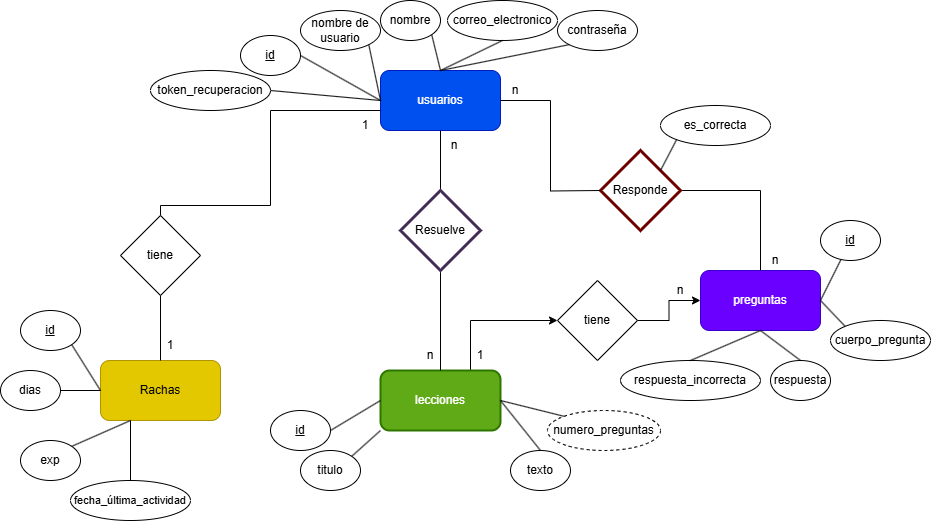
\includegraphics[width=0.9\linewidth]{Imagenes/DB_RM.png}
  \caption{Modelo Entidad Relación}
  \label{fig:ER}
\end{figure}


\subsection{Modelo UML}

\begin{figure}[H]
  \centering
  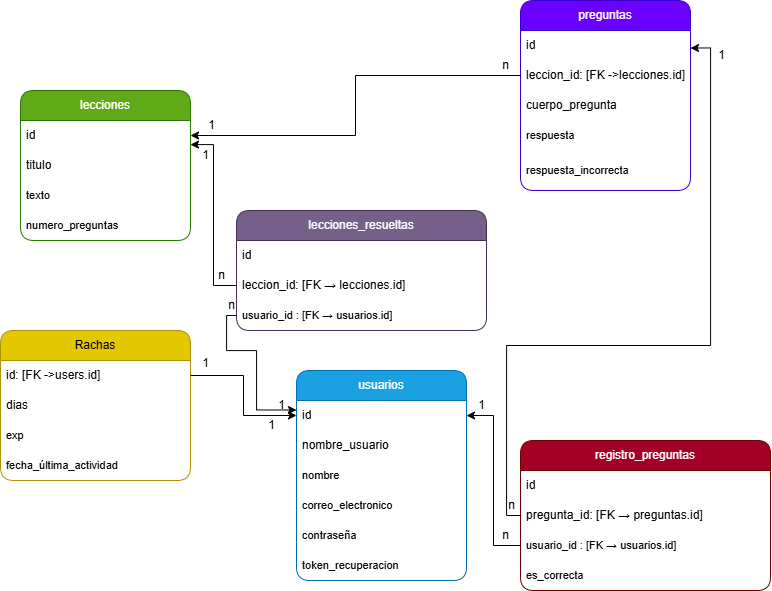
\includegraphics[width=0.6\linewidth]{Imagenes/DB_UML.png}
  \caption{Modelo UML}
  \label{fig:uml}
\end{figure}


\subsection{Base de datos NoSQL}

A diferencia de las bases de datos relacionales, Redis, al ser una base de datos NoSQL (Not Only SQL) no utiliza un esquema estructurado predefinido, ya que se basa en el almacenamiento de datos en formato clave-valor. Por esta razón, a continuación se detalla las claves utilizadas, los tipos de datos asociados y una breve descripción de su propósito dentro del sistema. Esta representación permite comprender la lógica de almacenamiento empleada en Redis y su papel en el prototipo.

\begin{table}[H]
\centering
\begin{tabular}{|p{3.5cm}|l|p{6cm}|}
\hline
\textbf{Tipo} & \textbf{Nombre de la variable} & \textbf{Descripci\'on} \\
\hline
Hash & \texttt{lesson:\{lesson\_id\}} & Almacena atributos de la lecci\'on: ID, t\'itulo y cantidad de preguntas. Esto con el objetivo de brindar en la pagina principal del prototipo una breve descripcion de todas las lecciones recientes. \\
\hline
Conjunto (set) & \texttt{all\_lessons} & Contiene todas las claves de lecciones creadas recientemente. Se utiliza para acceder a todas las lecciones actuales de forma eficiente. \\
\hline
Conjunto (set) & \texttt{user:\{user\_id\}:completed} & Guarda los ID de las lecciones completadas por un usuario espec\'ifico. Facilita brindar al usuario solo las lecciones actuales que tiene pendientes por realizar. \\
\hline
\end{tabular}
\caption{Estructuras de datos utilizadas en Redis}
\label{table:EstructurasRedis}
\end{table}


\section{Interfaz de usuario (UI/UX)}

En esta sección se describe la interfaz de usuario en su diseño de mockups desarrolladas para la aplicación, las cuales fueron diseñadas utilizando la herramienta Figma. Durante el proceso de diseño se priorizó la experiencia del usuario, asegurando una navegación intuitiva y una estética coherente con los objetivos de la plataforma. Además, se implementó un enfoque responsive que permite que la interfaz se adapte adecuadamente a distintos tamaños de pantalla, garantizando una visualización óptima en dispositivos móviles, tabletas y computadoras de escritorio. A continuación, se detallan las principales secciones y componentes de la interfaz. Cabe resaltar que este no representa el diseño final de la aplicación, ya que siempre existe un margen de mejora y ajustes según la retroalimentación de los usuarios. Si desea ver todas las mockups del prototipo y su diseño final, dirigirse a los \hyperref[Anexos]{Anexos}.

\newpage
\subsubsection{Imágenes utilizadas}

Las imágenes utilizadas en este proyecto, incluyendo las insignias y la imagen de inicio de sesión, fueron generadas mediante la inteligencia artificial DALL·E de OpenAI. Según la política de contenido de OpenAI \cite{openaicondicionesuso}, los usuarios poseen los derechos sobre las imágenes que crean, incluyendo el derecho a reimprimir, vender y comercializar dichas imágenes, independientemente de si fueron generadas mediante créditos gratuitos o pagos. Por lo cual las imágenes utilizadas en la interfaz no tendrán problema por derechos de autor.

\begin{figure}[H]
  \centering
  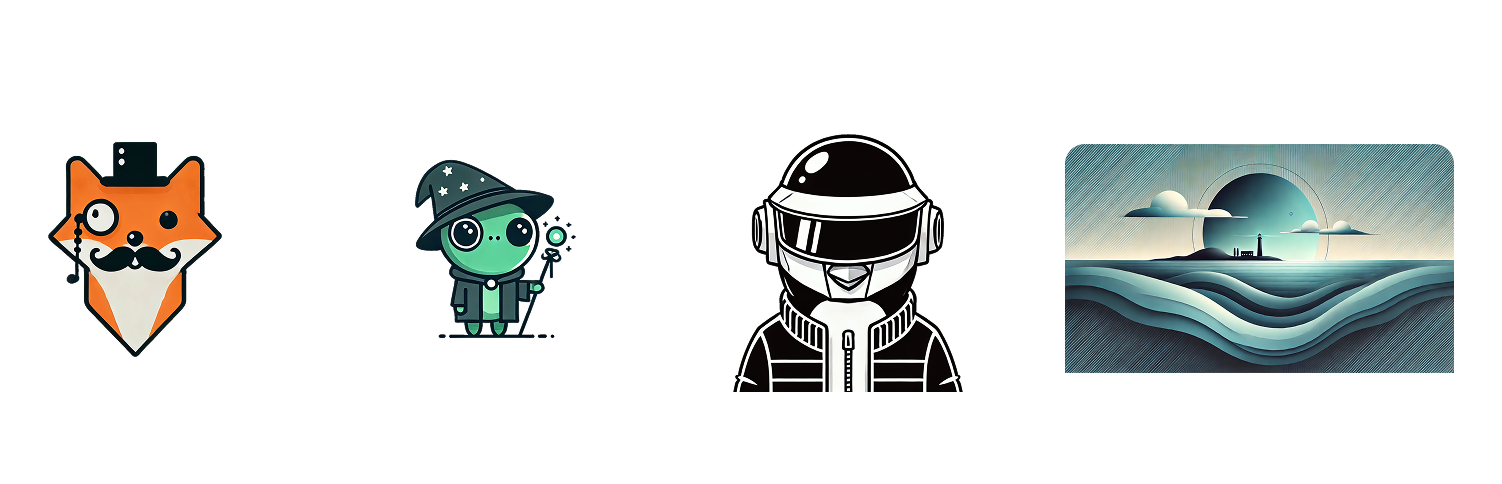
\includegraphics[width=0.8\linewidth]{Imagenes/Imagenes IA.png}
  \caption{Imágenes utilizadas}
  \label{fig:ER}
\end{figure}

\subsubsection{Módulo de logIn}

Este módulo permite el acceso de los usuarios que ya están registrados en el prototipo mediante correo electrónico y contraseña. La interfaz presenta un formulario simple, con campos identificados para el ingreso de credenciales. Además, se incluyen enlaces a las secciones “¿Olvidaste tu contraseña?” y “Regístrate”, que permiten respectivamente recuperar el acceso en caso de olvido y crear una nueva cuenta

\begin{figure}[H]
  \centering
  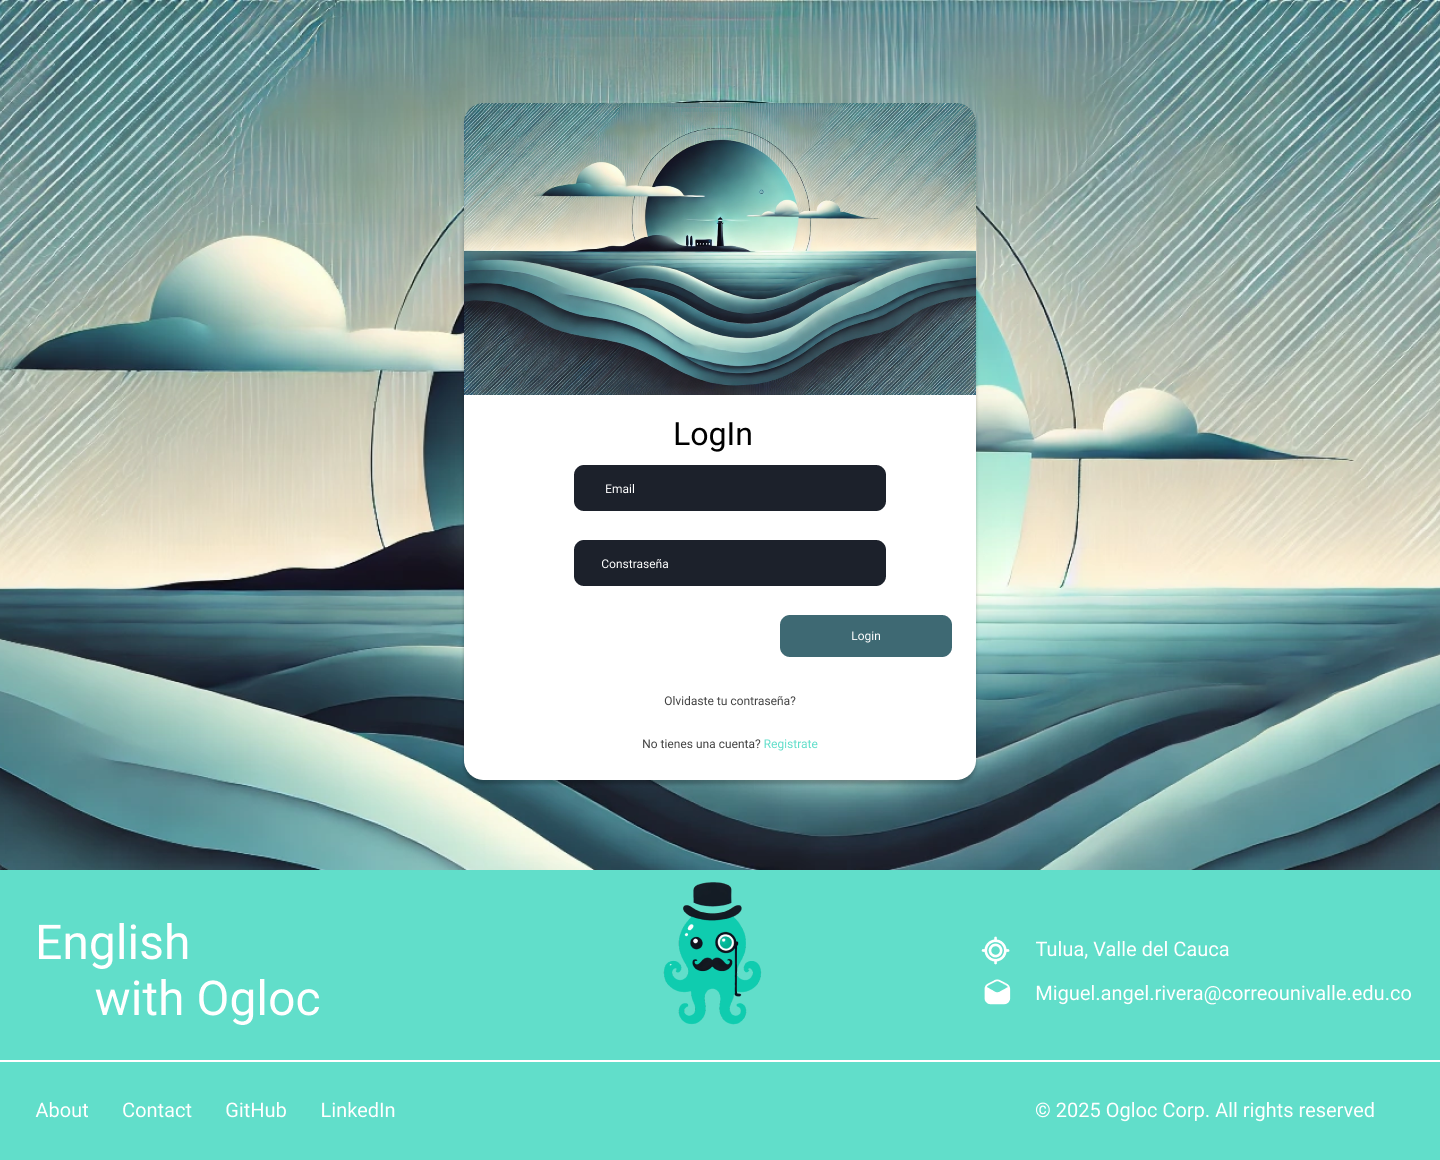
\includegraphics[width=0.8\linewidth]{Imagenes/Vista login.png}
  \caption{Mockup LogIn}
  \label{fig:ER}
\end{figure}

\subsubsection{Módulo de Registro}

El módulo de registro permite a los nuevos usuarios crear una cuenta en el prototipo mediante un formulario sencillo y accesible. Este formulario está compuesto por los campos: nombre completo, nombre de usuario (username), correo electrónico y contraseña. Cada uno de estos campos está diseñado para facilitar el ingreso de datos de manera clara y eficiente. Asimismo, se implementan validaciones básicas para asegurar que la información ingresada sea válida y coherente.

\begin{figure}[H]
  \centering
  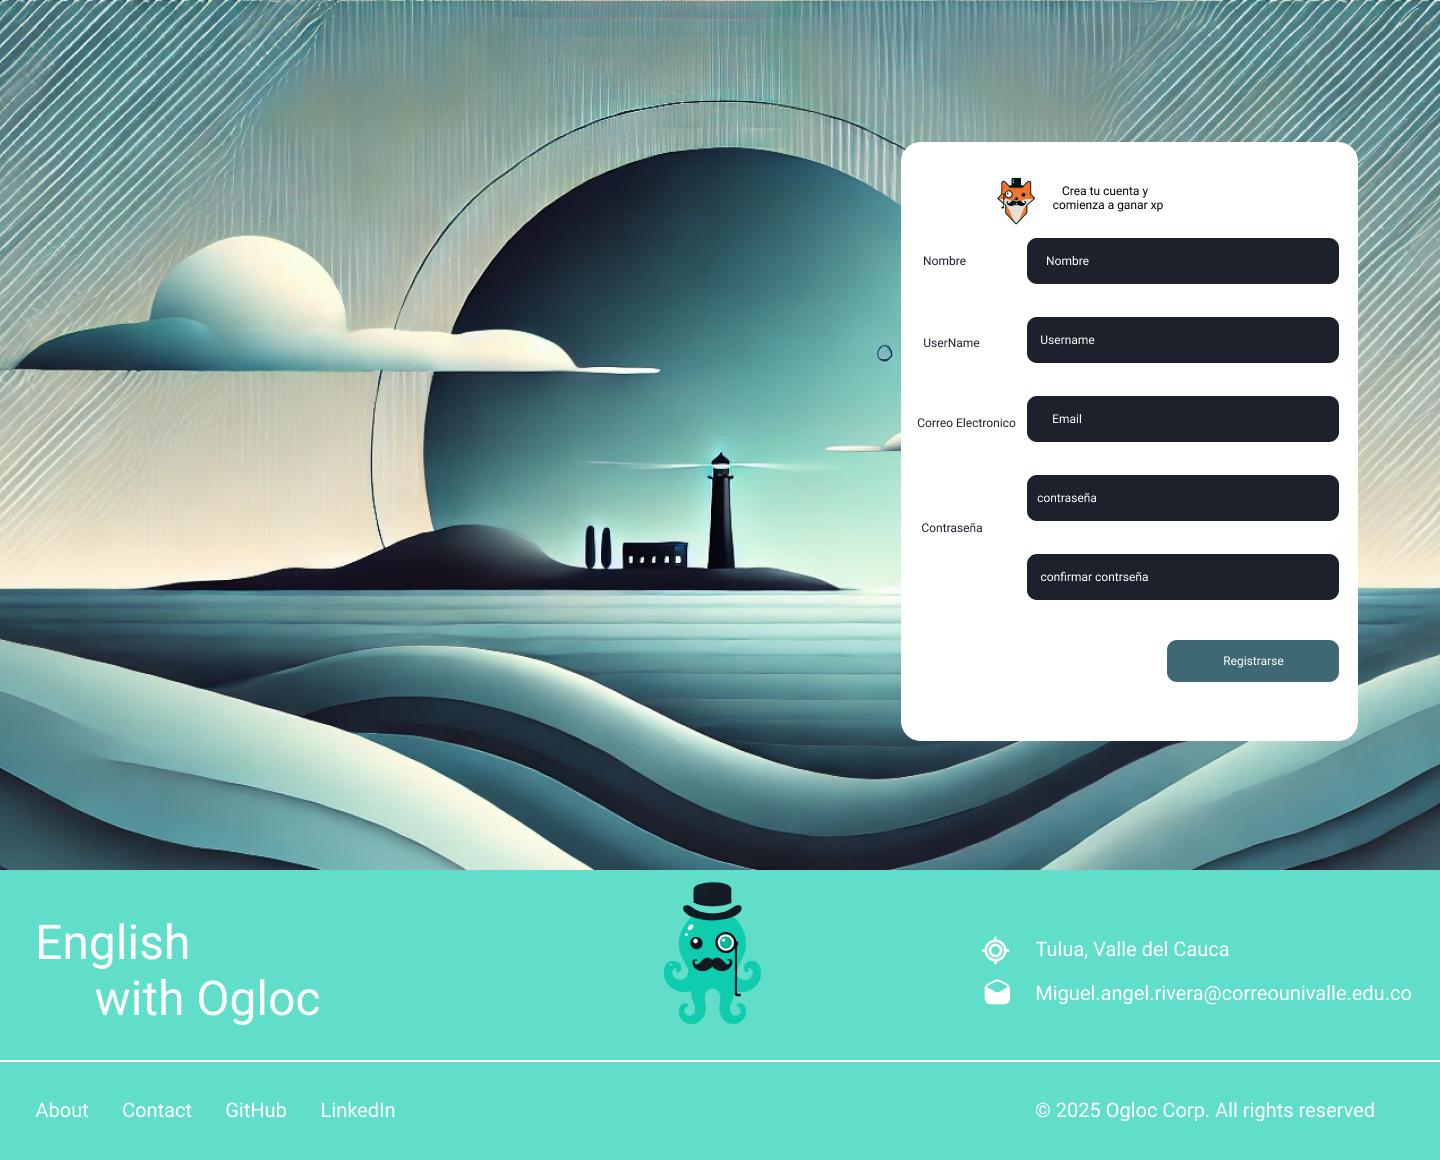
\includegraphics[width=0.6\linewidth]{Imagenes/Vista Registro.png}
  \caption{Mockup de Registro}
  \label{fig:ER}
\end{figure}


\subsubsection{Módulo perfil de usuario}

Este módulo permite al usuario visualizar y gestionar la información asociada a su cuenta. Desde esta sección, el usuario puede consultar datos como su nombre, nombre de usuario y su progreso dentro de la plataforma. Además, se incluye la posibilidad de editar algunos de estos datos o acceder a opciones adicionales como eliminar la cuenta.

\begin{figure}[H]
  \centering
  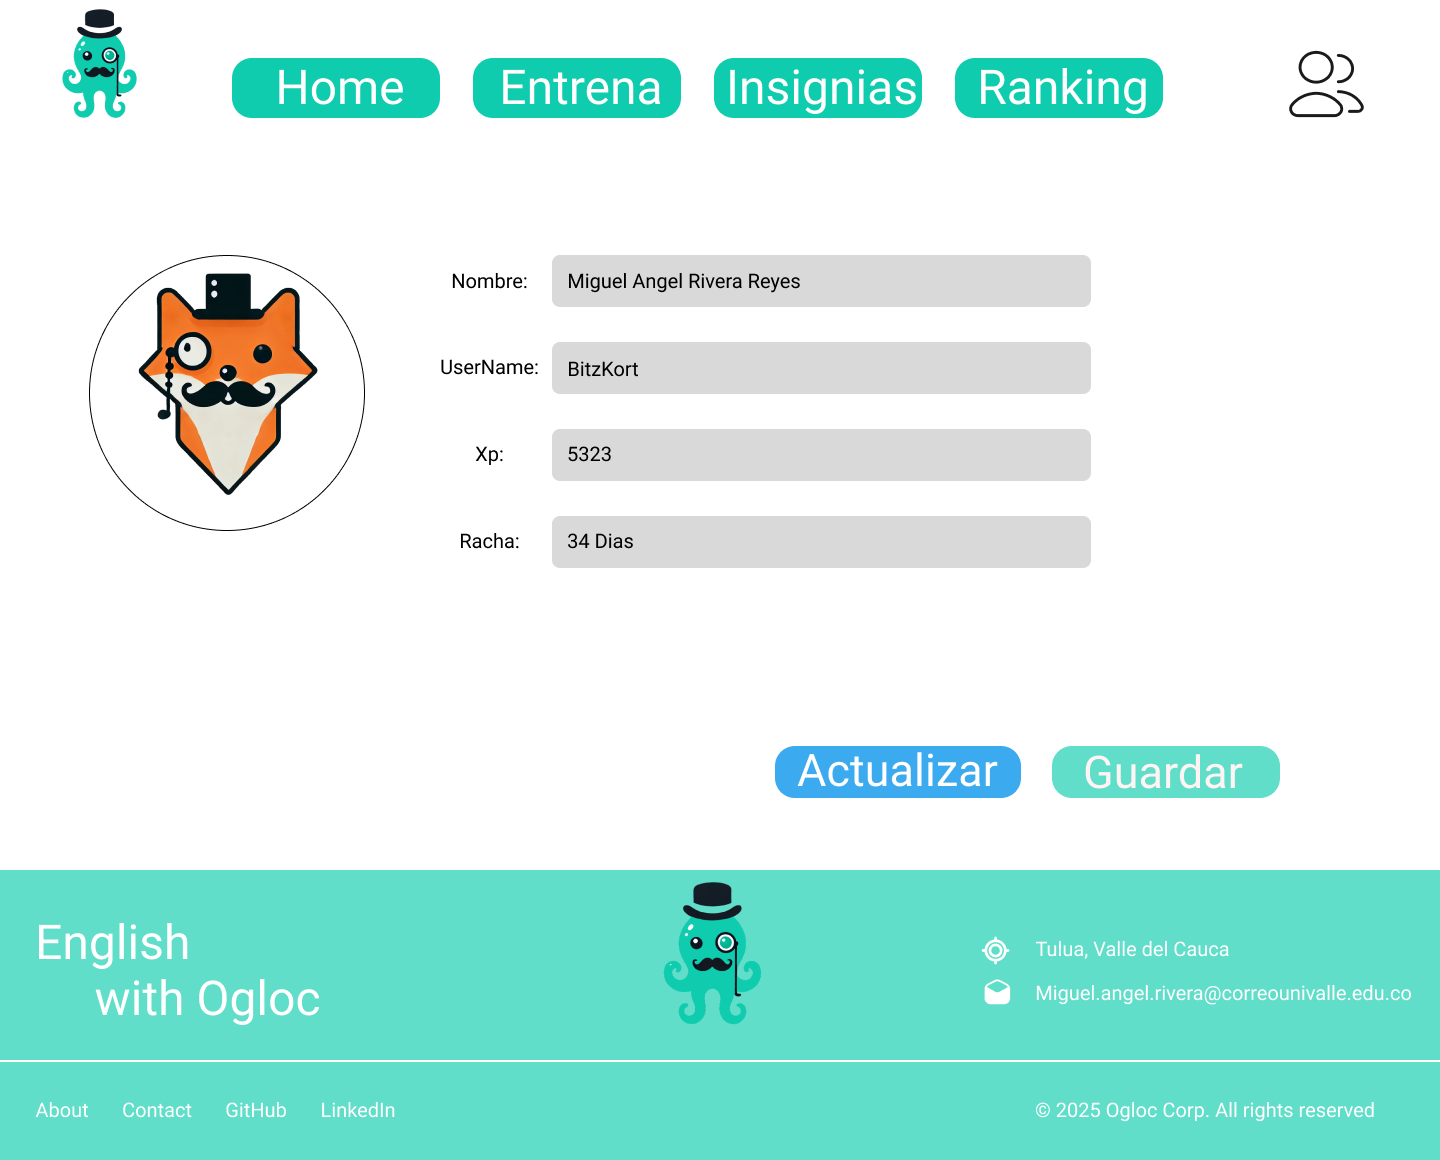
\includegraphics[width=0.5\linewidth]{Imagenes/vista perfil.png}
  \caption{Mockup perfil de usuario}
  \label{fig:ER}
\end{figure}

\subsubsection{Módulo preguntas}

Este módulo corresponde a la vista en la que se presentan las preguntas de cada lección , el usuario interactúa directamente con el contenido de aprendizaje respondiendo las preguntas que conforman una lección por medio del micrófono. Las preguntas se muestran una a una, de forma clara y ordenada.

\begin{figure}[H]
  \centering
  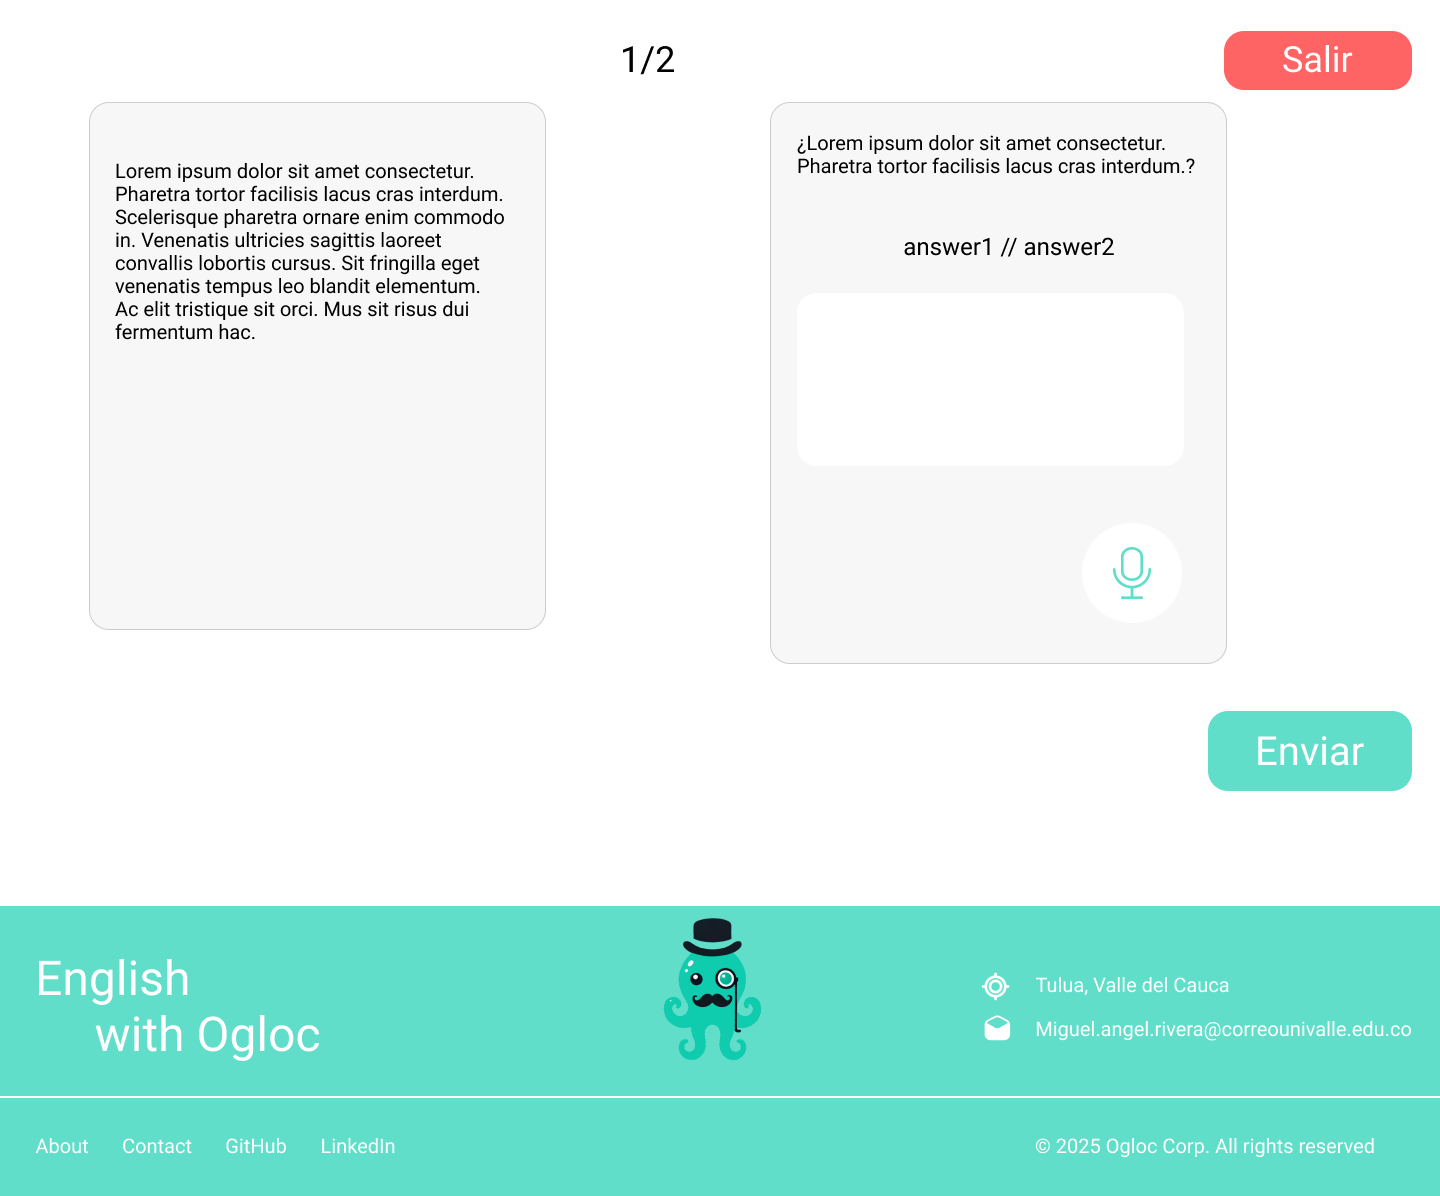
\includegraphics[width=0.6\linewidth]{Imagenes/Vista preguntas.png}
  \caption{Mockup vista preguntas}
  \label{fig:ER}
\end{figure}

\subsubsection{Módulo principal (home)}

Este módulo representa la página principal del prototipo, donde el usuario puede visualizar de forma general las funcionalidades más relevantes de la aplicación. En esta vista se presentan las lecciones disponibles para realizar, organizadas de manera que faciliten su acceso y comprensión. Además, se incluyen secciones dedicadas a las insignias obtenidas por el usuario, así como un acceso al pool de preguntas incorrectas, lo que permite reforzar los conocimientos previamente evaluados. Finalmente, se muestra un ranking global con los usuarios que han acumulado mayor experiencia (exp), promoviendo la motivación y el sentido de competencia entre los participantes.


\begin{figure}[H]
  \centering
  \includegraphics[width=0.5\linewidth]{Imagenes/Vista home.png}
  \caption{Mockup home}
  \label{fig:ER}
\end{figure}

\newpage
\subsubsection{Módulo Insignias}

Este módulo está dedicado a la visualización de las insignias que el usuario ha obtenido a lo largo de su progreso en la plataforma. Las insignias se otorgan en función de la cantidad de experiencia (exp) acumulada, la cual se incrementa a medida que el usuario responde correctamente las preguntas de las lecciones. Este sistema de recompensas tiene como objetivo incentivar la participación constante y reconocer el esfuerzo del usuario, proporcionando una representación visual de sus logros dentro de la aplicación. Las insignias se muestran de manera ordenada, permitiendo identificar tanto las obtenidas como las que aún están por desbloquear.

\begin{figure}[H]
  \centering
  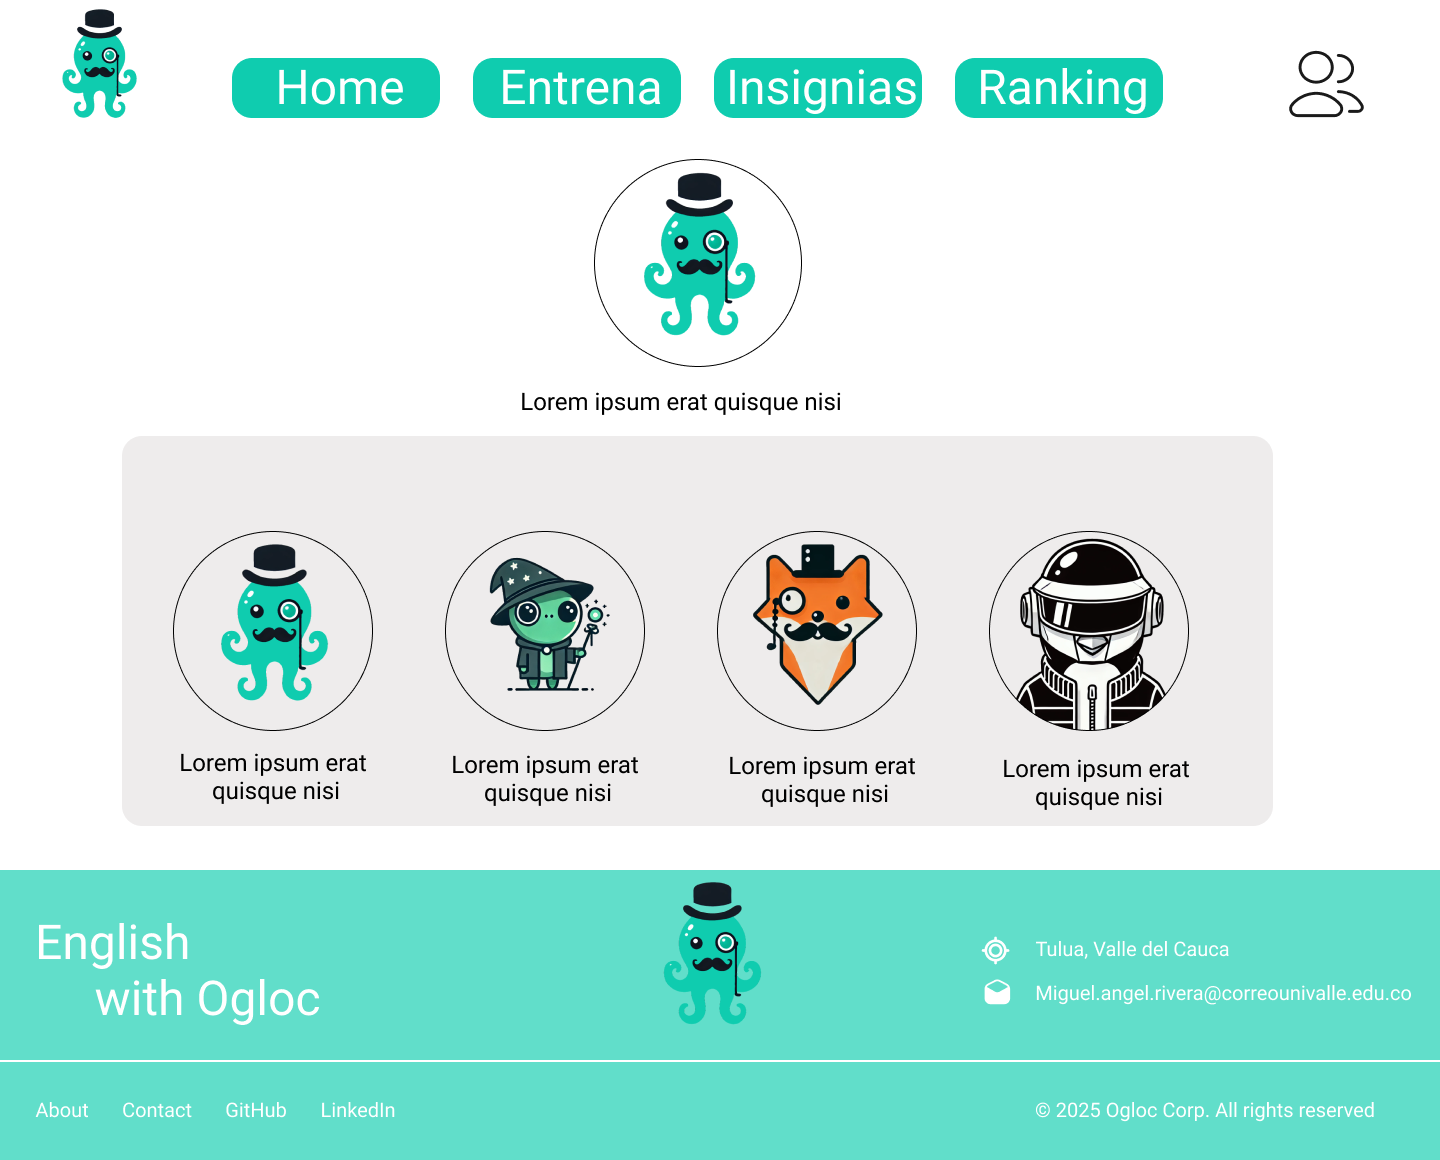
\includegraphics[width=0.6\linewidth]{Imagenes/Vista insignias.png}
  \caption{Mockup vista Insignias}
  \label{fig:ER}
\end{figure}

\newpage
\section{Diagrama de despliegue}

En el siguiente diagrama de arquitectura o de despliegue, se pueden visualizar los diferentes componentes que comprende la arquitectura del sistema. El diagrama es una herramienta que se utiliza para demostrar como están distribuidos los componentes de software en los diferentes elementos de hardware de un sistema.

\begin{figure}[H]
  \centering
  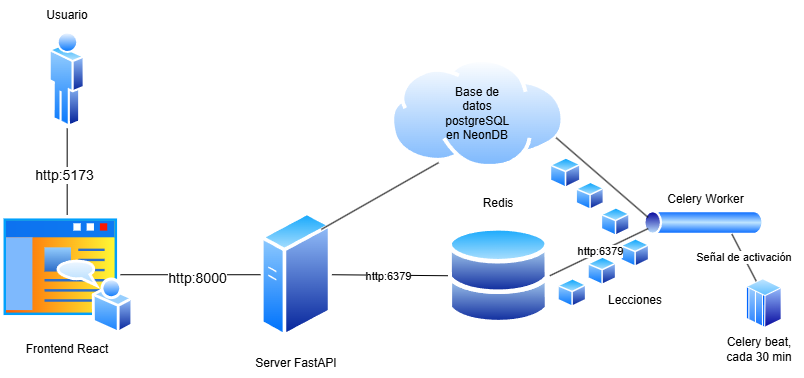
\includegraphics[width=0.9\linewidth]{Imagenes/Diagrama de despliegue.png}
  \caption{Diagrama de despliegue}
  \label{fig:ER}
\end{figure}

%%%%%%%%%%%%%%%%%%%%%%%%%%%%%%% Capitulo 6 %%%%%%%%%%%%%%%%%%%%%%%%%%%%%%%

\chapter{Desarrollo del prototipo web}
\section{Metodología de Desarrollo}

En las primeras etapas del proyecto, se decidió implementar ClickUp como herramienta para la gestión de tareas y proyectos. Si bien ClickUp ofrece numerosas funcionalidades, lo que resulta valioso para equipos con requerimientos específicos, su complejidad generó desafíos importantes. La plataforma presentó una curva de aprendizaje significativa, lo que afectó el desarrollo y la eficiencia durante el inicio del proyecto.
\\
\\
Frente a estas dificultades, se optó por migrar a Jira, una herramienta con la que ya se tenía experiencia previa. Aunque Jira también requiere un período de adaptación, este resultó más manejable debido a la familiaridad con la plataforma. La transición a Jira permitió organizar las tareas de manera más efectiva y seguir el progreso del proyecto con claridad.
\\
\\
Por último, se implemento la metodología Scrumban junto a un tablero Kanban para hacer un seguimiento continuo de las historias de usuario, de esta forma se favoreció una organización más clara, garantizando la correcta gestión de las historias de usuario del prototipo.

\subsection{Historias de usuario}

Las historias de usuario son descripciones cortas y claras que reflejan lo que el usuario final necesita o espera del sistema. Su objetivo es simplificar la comunicación entre todos los involucrados, asegurando que los requisitos queden bien entendidos y se implementen correctamente. En esta sección se detallan las historias de usuario que orientan el desarrollo del proyecto, explicando de forma precisa las funcionalidades y necesidades desde la perspectiva del usuario y del desarrollador. Cada historia está pensada para aportar un entendimiento general y especifico, garantizando que el producto cumpla con lo esperado durante el proceso de desarrollo.
\\
\\
A continuación se presentan dos historias de usuario como referencia, para ver todas las historias de usuario dirigirse a \hyperref[Anexos]{Anexos}.


\begin{table}[h!]
\centering
\renewcommand{\arraystretch}{2.2} % Aumenta la altura de las filas
\begin{tabular}{|>{\raggedright\arraybackslash}p{3cm}|m{10cm}|} % "m" centra verticalmente
  \hline
  \textbf{N\textdegree: 04} & Inicio de sesión \\ \hline
  \textbf{Descripci\'on} & Como usuario registrado quiero iniciar sesión con mi correo electrónico y contraseña para acceder al prototipo. \\ \hline
  \textbf{Tipo} &
    \begin{minipage}[c][2.2\baselineskip][c]{\linewidth}
      \centering
      Frontend \\ 
    \end{minipage} \\ \hline
  \textbf{Criterios de Aceptaci\'on} & \begin{itemize}
  \item Existe un formulario como una nueva p\'agina en el frontend con los campos:
  \begin{itemize}
    \item Email
    \item Contrase\~na
  \end{itemize}

  \item Al hacer clic en ``Iniciar sesi\'on'', el frontend env\'ia una petici\'on.
\end{itemize}  \\ \hline
\end{tabular}
\caption{Historia de usuario 4}
\end{table}


\begin{table}[H]
\centering
\renewcommand{\arraystretch}{2.2} % Aumenta la altura de las filas
\begin{tabular}{|>{\raggedright\arraybackslash}p{3cm}|m{10cm}|} % "m" centra verticalmente
  \hline
  \textbf{N\textdegree: 13} & Creación de rutas de autenticación \\ \hline
  \textbf{Descripci\'on} & Yo como desarrollador quiero definir y estructurar las rutas (endpoints) del servidor que realicen la tarea de autenticar el usuario para asegurar un acceso claro al prototipo. \\ \hline
  \textbf{Tipo} &
    \begin{minipage}[c][2.2\baselineskip][c]{\linewidth}
      \centering
      Backend \\
    \end{minipage} \\ \hline
  \textbf{Criterios de Aceptaci\'on} & \begin{itemize}
  \item Se deben implementar las siguientes rutas:
  \begin{itemize}
    \item Ruta para logIn.
    \item Ruta para registro de usuario.
    \item Ruta de recuperación de la contraseña (envío del email).
    \item Ruta para cambiar la contraseña (cambio real de la contraseña).
    \item Ruta para verificar el token en caso de cargar el logIn o el Registro en el frontend estando ya autenticado.
  \end{itemize}
  \item Cada ruta debe contener la lógica suficiente para ser funcional.
  \item Cada ruta debe estar protegida por el token JWT.
\end{itemize} \\ \hline
\end{tabular}
\caption{Historia de usuario 13}
\end{table}


\subsection{Tablero Scrumban}

Para gestionar y seguir con la metodología scrumban, se implemento un tablero Kanban que permite visualizar claramente cómo van las tareas. El tablero está dividido en varias secciones: "To Do", donde se listan las tareas que aún no se han iniciado; "In Progress", para las tareas que están en desarrollo; "Blocked", donde se colocan las tareas que enfrentan algún obstáculo que frena su progreso; "In Review", para las tareas que están siendo revisadas o validadas; y "Done", donde van las tareas finalizadas y aprobadas.

\begin{figure}[H]
  \centering
  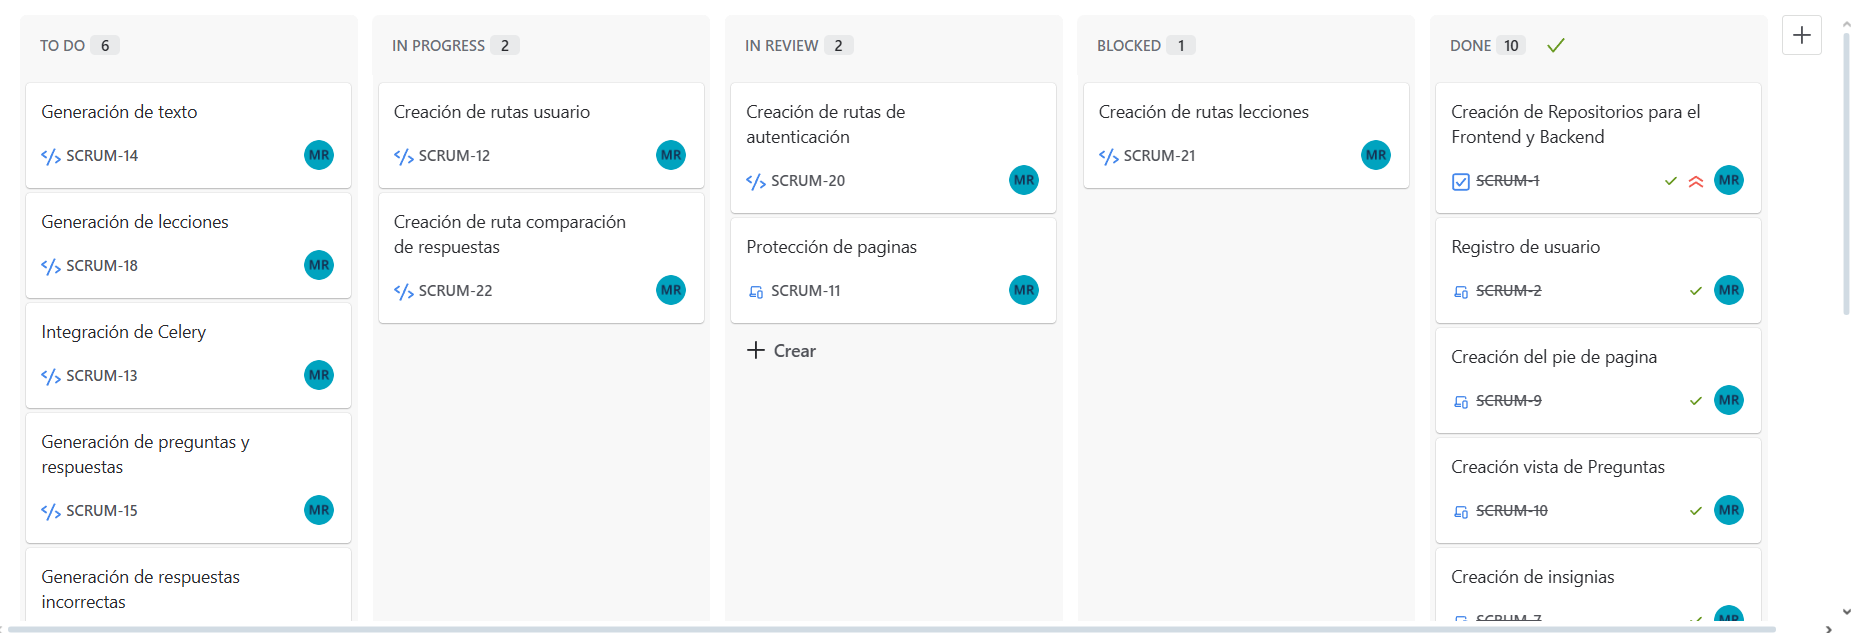
\includegraphics[width=1\linewidth]{Imagenes/tablero_tg.png}
  \caption{Tablero Scrumban}
  \label{fig:tablero}
\end{figure}



\input{capitulo6/Configuración_de_entornos}

\section{Arquitectura de generación de lecciones}

\subsection{Dataset Utilizado}

Para el desarrollo del prototipo y la generación de texto se empleó el dataset \texttt{wikipedia.20220301.simple}, el cual corresponde a artículos de Wikipedia (edición Simple English) con fecha del 1 de marzo de 2022. Este dataset contiene aproximadamente 205,328 artículos.

El procesamiento realizado se resume en los siguientes pasos:

\begin{enumerate}
  \item Se extrajo únicamente el primer párrafo de cada artículo, como representación más concisa del contenido.
  \item Se filtraron los textos para  descartar aquellos que contuvieran caracteres distintos al alfabeto latino básico (es decir, se eliminaron caracteres como acentos inusuales, alfabetos no latinos, símbolos extraños o de otros idiomas).
  \item Se construyó un nuevo dataset que incluye únicamente los campos: id, title y text, ajustados a los criterios anteriores.
  \item Por ultimo, el dataset final se guardó localmente para ser utilizado durante el desarrollo del prototipo.
\end{enumerate}

Gracias a estos filtros, garantizamos que cada artículo utilizado contenga únicamente caracteres válidos del alfabeto latino, lo cual resulta esencial para asegurar que la generación de texto incluyendo la respuesta correcta usada para comparar con la del usuario sea consistente, legible y libre de interferencias lingüísticas irrelevantes.

Después de aplicar estos filtros, se obtuvo un total de  120,703 artículos, los cuales conforman la base para la generación de texto a partir de este dataset.


\subsection{Modelo para generación de texto}
El modelo que se utilizo para generar texto es el modelo pre-entrenado de GPT-2, el cual está basado en la arquitectura de transformadores (transformers). Esta arquitectura se caracteriza por el uso del mecanismo de atención self-attention, que permite que cada palabra del texto se relacione con todas las demás de la secuencia. GPT-2 es un modelo auto-regresivo, lo que significa que genera texto palabra por palabra, prediciendo la siguiente palabra dado el contexto anterior. La clase implementa el patrón de diseño Singleton, el cual asegura que solo exista una única instancia activa del modelo en memoria durante la ejecución del programa.

\newpage
\subsubsection{Parámetros de Generación}
La clase utiliza el método pipeline de Hugging Face para configurar la generación de texto. Los principales parámetros usados son:

\begin{table}[H]
\centering
{\small
\begin{tabular}{|l|p{5cm}|p{5cm}|l|}
\hline
\textbf{Par\'ametro} & \textbf{Definici\'on} & \textbf{Efecto en la Generaci\'on} & \textbf{Valor} \\
\hline
\texttt{num\_beams} & Cantidad de caminos posibles que el modelo explora para encontrar el mejor resultado. & Mejora la calidad del texto al considerar varias opciones de generaci\'on al mismo tiempo. & 5 \\
\hline
\texttt{temperature} & Controla cu\'anta variedad puede tener el texto generado. & Un valor bajo hace el texto m\'as predecible; uno alto lo hace m\'as creativo y diverso. & 0.9 \\
\hline
\texttt{top\_k} & Limita la elecci\'on de palabras a las m\'as probables. & Ayuda a que el texto sea coherente al evitar palabras poco comunes o sin sentido. & 45 \\
\hline
\texttt{no\_repeat\_ngram\_size} & Evita que se repitan grupos de palabras del mismo tama\~no. & Hace que el texto se sienta m\'as natural al eliminar repeticiones innecesarias. & 3 \\
\hline
\end{tabular}
}
\caption{Par\'ametros de generaci\'on de texto en GPT-2}
\label{tab:parametros_gpt2}
\end{table}

\subsubsection{Procesamiento del Texto}

Por motivos de control y calidad del texto generado, el texto base (un articulo que este dentro del dataset ya procesado) es truncado a 70 caracteres, con el fin de adquirir un contexto mínimo sobre el cual generar texto. Ademas el texto generado pasa por una etapa de limpieza para garantizar un resultado coherente y legible:

\begin{enumerate}
    \item Se recorta el texto hasta el último signo de puntuación válido.
    \item Se eliminan caracteres no deseados mediante expresiones regulares.
    \item Se normalizan los espacios múltiples.
\end{enumerate}

\subsection{Modelos para generación de preguntas y respuestas}

Para el sistema de preguntas y respuestas se utilizaron dos modelos distintos, cada uno con un propósito específico. El modelo t5-large-generation-race-QuestionAnswer, basado en la arquitectura T5 y entrenado con el dataset RACE, se utilizó para la generación estructurada de preguntas y respuestas extractivas. Por otro lado, el modelo t5-large-generation-squad-QuestionAnswer, entrenado con el conjunto de datos SQuAD, se empleó para la generación estructurada de preguntas y respuestas abstractivas. Esta combinación permite ofrecer al usuario una experiencia más completa ya que debe de responder a preguntas cuya respuesta se encuentra explícitamente e implícitamente en el contenido dado, reforzando así tanto sus habilidades de comprensión como de interpretación.

\newpage
\subsubsection{Generaci\'on de preguntas}

Los dos modelos utilizados para la generaci\'on de preguntas y respuestas son basasados en la arquitectura T5 (Text-To-Text Transfer-Transformer). Esta arquitectura convierte todas las tareas de procesamiento de lenguaje natural en tareas de texto a texto, es decir, dado un texto de entrada, genera un texto de salida.
\\
\\
La clase \texttt{RaceModel} implementa el patr\'on de dise\~no Singleton para el modelo t5-large-generation-race-QuestionAnswer, el cual garantiza que solo exista una instancia activa del modelo en memoria durante la ejecuci\'on. Esto permite optimizar el uso de recursos, evitando la recarga del modelo cada vez que se desee generar una pregunta y su respectiva respuesta. De la misma manera la clase \texttt{SquadModel} implementa el patron singleton para el modelo t5-large-generation-squad-QuestionAnswer.

\subsubsection{Parámetros de Generación}

La generación de texto se realiza mediante el uso de la función pipeline de Hugging Face, que facilita la configuración de los modelos pre-entrenados. En el caso de ambos modelos, se configuraron los mismos parámetros que se describen en la \autoref {tab:parametros_gpt2} num beams = 5, temperature = 0.7, top k = 50 y no repeat ngram size = 2.

\subsubsection{Procesamiento de preguntas y respuestas}

Para asegurar la calidad del contenido generado, se realiza un proceso de limpieza. Esto incluye:

\begin{enumerate}
    \item Eliminación de caracteres no deseados mediante expresiones regulares.
    \item Recorte de espacios en blanco innecesarios y normalización.
\end{enumerate}

\subsection{Modelo para generación de respuestas incorrectas}

El modelo encargado de la generación de respuestas incorrectas se basa en una versión adaptada de T5 bajo el nombre t5-large-generation-race-Distractor. Este modelo fue configurado específicamente para generar opciones incorrectas plausibles a partir de una pregunta, una respuesta correcta y un contexto. Para su ejecución se carga mediante la clase  \texttt{DistractorModel} mas el uso del patrón singleton, lo que garantiza que sólo se mantenga una instancia activa en memoria, optimizando el uso de recursos.
\\
\\
Durante la generación de preguntas incorrectas, se configuraron los mismos parámetros que se describen en la \autoref {tab:parametros_gpt2} num beams=5, no repeat ngram size=2, temperature=0.9 y top k=50. La entrada al modelo se construye uniendo la pregunta, la respuesta correcta y el contexto, el cual es el texto generado por gpt2.

\newpage
\section{Flujo completo de generación de lecciones}

Para iniciar el flujo de generación de lecciones, se utiliza \texttt{Celery Beat}, un componente de Celery que permite programar tareas periódicas. En este caso, la tarea principal llamada \texttt{generate\_lessons} se ejecuta cada 30 minutos. Esto se define en la configuración mediante la clave \texttt{beat\_schedule}, especificando el uso del metodo \texttt{crontab(minute='\*/30')}.

\subsection{Inicialización de Workers}
Al iniciar cada proceso worker, se ejecuta la función \texttt{init pools}, la cual asigna una semilla de generación pseudoaleatoria distinta a cada uno, evitando así patrones repetitivos en la generación.
\\
\\
Esta estrategia es especialmente importante dado que Celery, por defecto, utiliza un pool prefork para la ejecución de tareas. El modo prefork consiste en la creación de múltiples procesos hijos a partir del proceso principal. Esto permite ejecutar tareas en paralelo aprovechando múltiples núcleos del CPU, pero también introduce ciertas consideraciones en la inicialización del estado interno de cada worker. Todos los procesos hijos heredan el estado de la memoria del proceso padre en el momento del \texttt{fork()}. Esto incluye el estado del generador de números pseudoaleatorios, lo que significa que sin una inicialización manual, todos los procesos hijos comenzarán con la misma semilla aleatoria y, por tanto, producirán secuencias idénticas de números pseudoaleatorios, lo cual afecta directamente a la generación de lecciones, generando las mismas lecciones por ciclo de trabajo.

\begin{figure}[H]
  \centering
  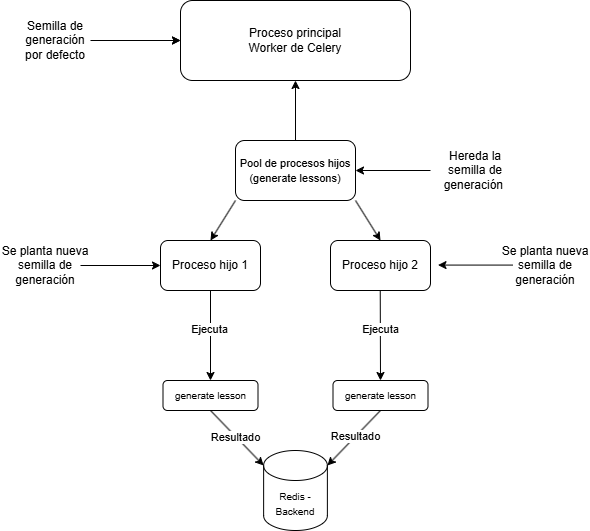
\includegraphics[width=0.7\linewidth]{Imagenes/diagrama de perfork.png}
  \caption{Diagrama de pool prefork en Celery}
  
  \label{fig:prefork}
\end{figure}

Para evitar este problema, como podemos ver en la figura~\ref{fig:prefork}, se utiliza la función \texttt{init pools} la cual se ejecuta justo después de que un proceso Worker ha sido inicializado y está listo para comenzar a ejecutar tareas. Dentro de init pools se realiza la lógica correspondiente para generar una semilla única con el método \texttt{random.seed()} realizando una combinación del PID (Process Identifier) del proceso (\texttt{os.getpid()}) y la marca de tiempo actual (\texttt{time.time()}). Con esto se garantiza que cada proceso tenga una secuencia única, evitando que se generen las mismas lecciones en cada ciclo.

\subsection{Tarea principal: generate lessons}
La tarea \texttt{generate lessons} es el punto de entrada del flujo. Esta tarea obtiene 6 muestras de texto desde el dataset previamente cargado usando la función \texttt{getDatasetText}.
\\
\\
A partir de estas muestras, se crean subtareas independientes mediante la tarea \texttt{generate\_lesson}, que son agrupadas y ejecutadas en paralelo. Una vez todas las lecciones han sido generadas, sus resultados se pasan a la tarea \texttt{save\_on\_dbs} para su almacenamiento.

\subsection{Generación de lecciones: generate\_lesson}
Cada subtarea de generación de lecciones sigue un proceso detallado:

\begin{enumerate}
\item Se genera un nuevo texto extendido a partir del texto de muestra usando un modelo basado en GPT-2 (\texttt{Gpt2Model}).
\item Si el texto generado tiene menos de 150 caracteres, se considera inválido y se re-intenta la tarea con una nueva muestra.
\item Se generan dos pares de pregunta-respuesta: uno usando el modelo RACE (\texttt{RaceModel}) y otro con el modelo SQuAD (\texttt{SquadModel}). Las preguntas y respuestas se separan usando el método \texttt{split\_qa}.
\item Para cada par de pregunta-respuesta, se genera una respuesta distractora utilizando el modelo \texttt{DistractorModel}. Si el distractor es igual a la respuesta, se re-intenta la generación.
\item Si todos los pasos son exitosos, se construye un objeto \texttt{LessonData} que agrupa el texto generado y las preguntas con sus respectivas respuestas y respuesta distractora.
\end{enumerate}

\subsection{Almacenamiento en bases de datos: save\_on\_dbs}
Una vez finalizadas todas las tareas de generación, los datos generados son almacenados en dos bases de datos:

\begin{itemize}
\item \textbf{Redis}: donde se guarda información ligera de cada lección en las estructuras definidas en la tabla \ref{table:EstructurasRedis}.
\item \textbf{PostgreSQL (NeonDB)}: donde se almacenan las preguntas y lecciones completas, manteniendo integridad referencial entre ellas.
\end{itemize}

Antes de realizar el guardado, se eliminan las lecciones anteriores con el propósito de que el usuario solo interactuare con las ultimas lecciones generadas.

\section{Repositorios}

 Puede encontrar el repositorio del frontend y el backend en github, a travez de los siguientes links:

\begin{itemize}
\item \textbf{Repositorio del backend:} \
\url{https://github.com/BitzKort/Trabajo-de-Grado-Backend}
\begin{itemize}
    \item Rama fastapiServer.
    \item Rama Celery.
\end{itemize}
\item \textbf{Repositorio del frontend:} \
\url{https://github.com/BitzKort/Ogloc-Frontend-TG}
    \begin{itemize}
    \item Rama main
    \end{itemize}
\end{itemize}




%%%%%%%%%%%%%%%%%%%%%%%%%%%%%%% Capitulo 7 %%%%%%%%%%%%%%%%%%%%%%%%%%%%%%%

\chapter{Pruebas sobre el prototipo}
\section{Justificación de las Pruebas}

Todas las encuestas incluidas en esta sección, junto con sus respectivos gráficos se encuentran a disposición en \hyperref[Anexos]{Anexos}.

\subsection{Encuesta: Impacto del Dominio del Inglés en la Vida Académica y Profesional}

Este formulario se diseñó con el propósito de analizar el impacto que tiene el dominio (o su ausencia) del inglés en la vida académica y profesional de las personas. Se busca validar la idea de que la competencia idiomática influye significativamente en el acceso a nuevas oportunidades tanto académicas, profesionales y sociales.

\subsection{Encuesta: Prueba de usabilidad English with Ogloc}

Se diseño el cuestionario para evaluar la usabilidad del prototipo web. El objetivo es verificar la efectividad de la interfaz de usuario  y sus principales funciones, como lo son las técnicas de gamificación utilizadas y la generación de lecciones. Ademas, con el fin de evaluar la generación de nuevas lecciones, se estableció un intervalo de generación de 30 minutos para que los encuestados interactúen con distintas lecciones.

\subsection{Encuesta: Prueba sobre niveles de ingles English with Ogloc}

Este formulario tiene como objetivo evaluar la calidad de todo el texto generado (incluyendo preguntas y respuestas) generados por el prototipo. La encuesta está dirigida a docentes especializados en la enseñanza del inglés, por ende esto permite garantizar la validez del contenido generado. Ademas su  aplicación contribuye directamente al cumplimiento del objetivo específico 1 del proyecto, pues se valida que las lecciones generadas dentro del prototipo están a un nivel de ingles B1. Se toma como referencia los descriptores del nivel B1 del Marco Común Europeo de Referencia para las Lenguas (MCER), asegurando así que los encuestados tengan su definición para realizar una evaluación adecuada.

\subsection{Encuesta: Prueba de usabilidad basada en las Heurísticas de Jakob Nielsen}

Esta encuesta se realiza con la finalidad de evaluar la usabilidad del prototipo, enfocándose en la calidad de la interfaz de usuario. En particular, se busca determinar cuán agradable y fácil de usar resulta la aplicación para los usuarios.

\section{Resultados y Análisis}

\subsection{Resultados: Impacto del Dominio del Inglés en la Vida Académica y Profesional}

A continuación se mostraran las preguntas de la encuesta Impacto del Dominio del Inglés en la Vida Académica y Profesional.

\begin{enumerate}
\item[\textbf{1.}] \textbf{\textquestiondown Hasta qué punto consideras que la falta de conocimientos en el idioma inglés ha afectado tu rendimiento académico?}\\\\
Escala de respuesta: 1 (No ha afectado en absoluto) -- 5 (Ha afectado en gran medida)\\ 

\textbf{Resultados: } el 34.6\%  (votos entre la escala 4 y 5) contesto que si los ha afectado significativamente, el 42.3\% (votos en la escala 3) contesto que  no afecto su rendimiento académico , el 19.2\% (votos en la escala 2) contesto que no les afecto significativamente y el 3.8\% (votos en la escala 1) contesto que no les afecto en lo absoluto.
\\
\item[\textbf{2.}] \textbf{\textquestiondown Qué tan complicado ha sido para tu vida personal (por ejemplo, acceder a oportunidades, comunicarse en viajes o en redes sociales) el no dominar adecuadamente el inglés?}\\\\
Escala de respuesta: 1 (Nada complicado) -- 5 (Muy complicado)\\

\textbf{Resultados: } el 57.7\% (votos entre la escala 4 y 5) contesto que si ha sido complicado, el 34.6\% (votos en la escala 3) contesto de forma neutral y el 7.7\% (votos en la escala 2) contesto que no ha sido complicado significativamente.
\\
\item[\textbf{3.}] \textbf{\textquestiondown En qué medida consideras que el uso de herramientas de Procesamiento de Lenguaje Natural (PLN) podría mejorar la calidad del aprendizaje en el aula de inglés?}\\\\
Escala de respuesta: 1 (No mejoraría) -- 5 (Mejoraría en gran medida))\\

\textbf{Resultados: } el 84.6\% (votos en la escala 4 y 5) contesto que si mejoraría significativamente, mientras que el 15.4\% (votos en la escala de 3) contesto de forma neutral.
\\
\end{enumerate}

\subsection{Análisis: Impacto del Dominio del Inglés en la Vida Académica y Profesional}

Los resultados de esta encuesta confirman que el dominio del inglés tiene un impacto relevante en la vida académica y personal de los individuos. Esto se evidencia en que el 34.6\% de los encuestados afirmó que la falta de conocimientos en inglés ha afectado significativamente su rendimiento académico, mientras que el 42.3\% manifestó un impacto moderado. Además, el 57.7\% indicó que la ausencia de dominio del inglés ha dificultado aspectos de su vida personal, como acceder a oportunidades, viajar o comunicarse en redes sociales. Finalmente, se observa una fuerte aceptación hacia el uso de tecnologías para el aprendizaje de idiomas, ya que el 84.6\% de los participantes considera que las herramientas de Procesamiento de Lenguaje Natural (PLN) mejorarían significativamente el aprendizaje del inglés en el aula. Estos resultados  refuerzan la justificación del proyecto y respaldan la necesidad de desarrollar soluciones tecnológicas innovadoras que ayuden a cerrar la brecha idiomática en contextos educativos.


\subsection{Resultados:  Prueba de usabilidad English with Ogloc}

A continuación se mostraran las preguntas de la encuestas:

\begin{enumerate}
\item[\textbf{1.}] \textbf{\textquestiondown Te resultó fácil acceder y completar las nuevas lecciones generadas automáticamente durante el periodo de prueba?}\\\\
Opciones de respuesta: Sí / No\\

\textbf{Resultados: } el 100\% de los encuestados les resulto fácil acceder y completar las nuevas lecciones
\\
\item[\textbf{2.}] \textbf{\textquestiondown Qué te parece la generación de nuevas lecciones en intervalos de tiempo definidos (en este caso, cada 30 minutos)?} \\\\
Escala de respuesta: 1 (Poco adecuado) -- 5 (Muy adecuado)\\

\textbf{Resultados: } el 86.6\% (votos entre la escala 4 y 5) contesto que el tiempo de 30 minutos fue muy adecuado, mientras que el 34.3\% (votos en la escala 4) contesto que el tiempo fue adecuado y el 11.4\% (votos en la escala 3) contesto de forma neutral.
\\
\item[\textbf{3.}] \textbf{\textquestiondown Qué te parecieron las preguntas incluidas en las lecciones generadas por el prototipo?}\\\\
Escala de respuesta: 1 (Poco claras) -- 5 (Muy claras)\\

\textbf{Resultados: } el 85.7\% (votos entre la escala 4 y 5) contesto que las preguntas fueron muy claras, mientras que el 14.3\% (votos en la escala 3) contestaron de forma neutral.
\\
\\
\item[\textbf{4.}] \textbf{\textquestiondown Qué tan motivado/a te sentiste al ver tu progreso reflejado (cambio de insignias, aumento de puntos de experiencia) dentro del prototipo?}\\\\
Escala de respuesta: 1 (Poco motivado) -- 5 (Muy motivado)\\


\textbf{Resultados: } el 91.4\% (votos entre la escala 4 y 5) contesto que si se sintieron mu motivados, mientras que el 5.7\% (votos en la escala 3) contesto de forma neutral y el 2.9\% contesto que no se sintieron motivados significativamente.
\\
\item[\textbf{5.}] \textbf{\textquestiondown Crees que las recompensas (como insignias y puntos de experiencia) reflejan adecuadamente tu desempeño y esfuerzo?} \\\\
Opciones de respuesta: S\'i / No\\

\textbf{Resultados: } el 94.3\% contesto que Si reflejan el desempeño y esfuerzo, mientras que el 8.6\% contesto que no.
\\

\item[\textbf{6.}] \textbf{\textquestiondown Qué tan fácil te resultó utilizar el micrófono para responder las preguntas del prototipo?}\\\\
Escala de respuesta: 1 (Muy complicado) -- 5 (Muy fácil)\\

\textbf{Resultados: } el 94.3\% ( votos entre la escala 4 y 5) contesto que si fue fácil utilizar el micrófono, mientras que el 5.7\% (votos en la escala 3) contesto de forma neutral.
\\
\item[\textbf{7.}] \textbf{\textquestiondown Qué tan bien se adaptó la interfaz del prototipo al tamaño de pantalla que usaste?}\\\\
Opciones de respuesta: Muy mal / Neutro / Muy bien\\

\textbf{Resultados: } el 74.3\% contesto que la interfaz del prototipo se adapto muy bien, mientras que el 25.7\% contesto de forma neutral.
\\
\item[\textbf{8.}] \textbf{\textquestiondown Los elementos visuales (botones, menús, texto, insignias) se mostraban correctamente en el tamaño de pantalla que usaste?} \\\\
Opciones de respuesta: Sí / No\\

\textbf{Resultados: } el 94.3\% contesto que si se mostraban correctamente, mientras que el 8.6\% contesto que no.
\\
\end{enumerate}

\newpage
\subsection{Análisis: Prueba de usabilidad English with Ogloc}

Los resultados de esta encuesta demuestran que el prototipo web presenta un alto nivel aceptación por parte de los usuarios. En primer lugar, el 100\% de los encuestados indicó que les resultó fácil acceder y completar las lecciones generadas automáticamente, lo cual refleja una interfaz intuitiva y sin barreras de acceso. Además, el 86.6\% consideró muy adecuado el intervalo de 30 minutos para la generación de nuevas lecciones, validando la estrategia temporal implementada.
\\
\\
Respecto al contenido, el 85.7\% opinó que las preguntas eran muy claras, lo que indica que la formulación de los ejercicios fue efectiva y comprensible para los usuarios. En cuanto a la gamificación, el 91.4\% se sintió muy motivado al ver su progreso reflejado en forma de insignias y puntos de experiencia, y el 94.3\% consideró que estas recompensas representaban adecuadamente su esfuerzo, lo que evidencia un diseño motivador y justo.
\\
\\
El uso del micrófono para responder preguntas fue calificado como muy fácil por el 94.3\% de los encuestados, mostrando que la integración fue exitosa. En cuanto al diseño responsivo, el 74.3\% afirmó que la interfaz se adaptó muy bien al tamaño de su pantalla, y el 94.3\% confirmó que los elementos visuales se mostraban correctamente. Estos resultados indican que el prototipo ofrece una muy buena experiencia de usuario, lo que lleva a que estos datos respalden la efectividad del prototipo en términos accesibilidad, claridad en los contenidos y motivación mediante elementos de gamificación.


\subsection{Resultados: Prueba sobre niveles de ingles English with Ogloc}

Cabe de resaltar que esta encuesta al ser para profesores de ingles, su población es muy reducida (3 encuestados) por lo que los porcentajes están bastante altos, sin embargo por eso mismo, al ser académicos con estudios en la enseñanza del idioma ingles, saben identificar con claridad si un texto cumple con el nivel objetivo que se esta evaluando. Ademas son profesores activos en su profesión, por lo que poseen su conocimiento fresco en una aplicación constantemente.

\begin{enumerate}
\item[\textbf{1.}] \textbf{\textquestiondown Consideras que los textos generados están dentro del nivel B1 de inglés?}\\\\
Opciones de respuesta: Sí / No\\

\textbf{Resultados: } el 100\% de los encuestados considera que los textos generados están dentro de un nivel de ingles B1.
\\

\item[\textbf{2.}] \textbf{\textquestiondown Las preguntas formuladas son acordes al contenido de los textos?}\\\\
Opciones de respuesta: Sí / No\\

\textbf{Resultados: } el 100\% contesto que las preguntas si son acordes al contenido de los textos generados.
\newpage
\item[\textbf{3.}] \textbf{\textquestiondown Qué tan apropiada te pareció la complejidad gramatical de los textos para el nivel B1?}\\\\
Opciones de respuesta: Demasiado simple / Demasiado complejo / Perfectamente adecuada\\

\textbf{Resultados: } el 100\% contesto que le pareció adecuada la complejidad gramatical de los textos para el nivel B1.
\\

\item[\textbf{4.}] \textbf{\textquestiondown En qué medida consideras que la estructura de las lecciones (un texto seguido de dos preguntas) se ajusta a lo que se esperaría de un estudiante con nivel de inglés B1?}\\\\
Opciones de respuesta: \\
No se ajusta en absoluto / Se ajusta muy poco / Se ajusta de forma moderada / Se ajusta bastante / Se ajusta completamente\\

\textbf{Resultados: } el 66.7\% contesto que la estructura si se ajustaría completamente, mientras que el 33.3\% contesto que se ajusta bastante.
\\

\item[\textbf{5.}] \textbf{\textquestiondown En qué medida el vocabulario de los textos coincide con los contenidos temáticos enseñados hasta alcanzar el nivel B1?}\\\\
Escala de respuesta: 1 -- 5\\

\textbf{Resultados: } el 100\% de los encuestados contestaron que coincide completamente con los contenidos enseñados hasta B1.
\\

\item[\textbf{6.}] \textbf{\textquestiondown En qué medida recomendarías este prototipo a otras personas que deseen practicar su fluidez en inglés?} \\\\
Escala de respuesta: 1 (No lo recomendaría en lo absoluto) -- 5 (Lo recomendaría completamente)\\

\textbf{Resultados: } el 100\% recomendaría el prototipo a personas que deseen practicar su fluidez.
\\

\item[\textbf{7.}] \textbf{\textquestiondown Qué tan de acuerdo estás con la metodología de enseñanza propuesta, basada en la gamificación y el uso de tecnologías de Procesamiento de Lenguaje Natural como apoyo para el aprendizaje del inglés?} \\\\
Opciones de respuesta: En desacuerdo / Ni de acuerdo ni en desacuerdo / De acuerdo / Totalmente de acuerdo\\


\textbf{Resultados: } el 100\% contesto que esta de acuerdo con la metodología de enseñanza basada en gamificación y el uso de tecnologías de Procesamiento de Lenguaje Natural. 
\\

\end{enumerate}

\subsection{Análisis: Prueba sobre niveles de ingles English with Ogloc}

Los resultados de la encuesta a docentes de inglés demuestran una valoración altamente positiva del prototipo . El 100\% de los encuestados considera que los textos se ajustan adecuadamente al nivel B1, afirmaron que las preguntas formuladas son adecuadas respecto al contenido de los textos y que la estructura de las lecciones es apropiada para estudiantes de este nivel.
\\
\\
En cuanto a la estructura de las lecciones, la mayoría (66.7\%) señaló que la organización de las lecciones se ajusta completamente a lo esperado en el nivel B1, mientras que el 33.3\% opinó que se ajusta bastante. Todos los participantes coincidieron en que el vocabulario es adecuado y en que recomendarían el prototipo para quienes deseen practicar su fluidez en inglés. Además, hubo un consenso total sobre la pertinencia de la metodología basada en gamificación y el uso de tecnologías de Procesamiento de Lenguaje Natural, por ende  el prototipo cumple con los criterios lingüísticos requeridos para el nivel B1.


\subsection{Resultados: Prueba de usabilidad basada en las Heurísticas de Jakob Nielsen}

Cabe de resaltar que esta encuesta al ser para profesionales titulados de Ingeniería de Sistemas se vio afectada pues no se logro obtener mas de 6 encuestados, sin embargo al ser profesionales titulados de la carrera y con años de experiencia, los encuestados saben identificar con claridad si una interfaz de usuario del prototipo cumple o no con las siguientes preguntas:


\begin{enumerate}

\item[\textbf{1.}] \textbf{\textquestiondown La aplicación me informa claramente sobre lo que está sucediendo (por ejemplo, cuando está grabando, procesando o esperando)?} \\\\
Escala de respuesta: 1 (Nada claro) -- 5 (Muy claro)\\

\textbf{Resultados: } el 66.7\% (votos en la escala 5) de los encuestados respondieron que está muy claro, mientras que el 40\% (votos en la escala 4) contestó que está claro.
 \\

\item[\textbf{2.}] \textbf{\textquestiondown El lenguaje y los iconos utilizados en la aplicación son fáciles de entender y familiares para ti?} \\\\
Escala de respuesta: 1 (Nada comprensible) -- 5 (Muy comprensible)\\

\textbf{Resultados: } el 66.7\% (votos en la escala 5) indicó que el lenguaje y los iconos utilizados son muy comprensibles, mientras que el otro 33.3\% (votos en la escala 4) afirmó que son comprensibles.
\\

\item[\textbf{3.}] \textbf{\textquestiondown Puedes deshacer o cancelar acciones fácilmente si cometes un error?} \\\\
Escala de respuesta: 1 (Nada fácil) -- 5 (Muy fácil)\\

\textbf{Resultados: } el 50\% (votos en la escala 5) contesto que fue muy fácil, mientras que el 33.3\% (votos en la escala 4) contestaron que fue fácil, y el 16.7\% (votos en la escala 2) contesto que no fue tan fácil cancelar acciones si se comete un error.
\\

\item[\textbf{4.}] \textbf{\textquestiondown Los elementos de la interfaz (botones, menús, mensajes) son consistentes en toda la aplicación?} \\\\
Escala de respuesta: 1 (Nada consistentes) -- 5 (Muy consistentes)\\

\textbf{Resultados: } el 50\%(votos en la escala 5) contesto que los elementos de la interfaz son muy consistentes y el 50\% (votos en la escala 4) contesto que son algo consistentes, lo cual refleja una buena percepción sobre la interfaz.
\\

\item[\textbf{5.}] \textbf{\textquestiondown La aplicación te ayuda a evitar errores y te advierte antes de realizar acciones importantes?} \\\\
Escala de respuesta: 1 (No ayuda) -- 5 (ayuda mucho)\\

\textbf{Resultados: } el 16.7\% (votos en la escala 5) contesto que si ayuda mucho y el 83.3\% (votos en la escala 4) contesto que fue ayuda significativamente, reflejando una percepción positiva sobre la prevención de errores.
\\

\item[\textbf{6.}] \textbf{\textquestiondown La información y las opciones importantes están siempre visibles o fácilmente accesibles, sin necesidad de recordar pasos previos?} \\\\
Escala de respuesta: 1 (Nada accesibles) -- 5 (Muy accesibles)\\

\textbf{Resultados: } el 33.3\% (votos en la escala 5) indicó que la información es accesible y el 66.7\% (votos en la escala 4) consideró que es muy accesible.
\\

\item[\textbf{7.}] \textbf{\textquestiondown La aplicación permite realizar tareas de manera eficiente, tanto para usuarios nuevos como experimentados?} \\\\
Escala de respuesta: 1 (Nada eficiente) -- 5 (Muy eficiente)\\

\textbf{Resultados: } el 33.3\% (votos en la escala 5) contesto que fue muy eficiente y el 66.7\% (votos en la escala 4) contesto que fue algo eficiente, demostrando que la eficiencia y flexibilidad de uso es adecuada.
\\

\item[\textbf{8.}] \textbf{\textquestiondown La interfaz es clara, simple y no contiene información innecesaria?} \\\\
Escala de respuesta: 1 (Muy recargada) -- 5 (Muy minimalista)\\

\textbf{Resultados: } el 50\% (votos en la escala 5) contesto que la interfaz es muy minimalista, el 33.3\% (votos en la escala 4) contestaron que la interfaz es algo minimalista y el 16.7\% (votos en la escala 3) contesto de forma neutral, evidenciando una tendencia positiva hacia un diseño claro y funcional.
\\

\item[\textbf{9.}] \textbf{\textquestiondown Los mensajes de error son claros y te ayudan a entender cómo solucionar el problema?} \\\\
Escala de respuesta: 1 (Nada claros) -- 5 (Muy claros)\\

\textbf{Resultados: } el 33.3\% (votos en la escala 5) contesto que los mensajes de error son muy claros, y el 66.7\% (votos en la escala 4) contestaron que son algo claros,  mostrando buena respuesta a la gestión de errores
 \\
 
\item[\textbf{10.}] \textbf{\textquestiondown Si lo necesitas, puedes encontrar fácilmente ayuda o instrucciones sobre cómo usar la aplicación?} \\\\
Escala de respuesta: 1 (Nada accesible) -- 5 (Muy accesible)\\


\textbf{Resultados: } el 50\% (votos en la escala 5) contestaron que es muy accesible, el 33.3\% (votos en la escala 4) contestaron que es algo accesible y el 16.7\% (votos en la escala 1)  contesto que no es nada accesible, indicando que la ayuda y documentación están bien implementadas sin embargo se debe reforzar levemente.
\\
\end{enumerate}


\subsection{Análisis: Prueba de usabilidad basada en las Heurísticas de Jakob Nielsen}

La prueba de usabilidad basada en las heurísticas de Nielsen, fue aplicada a un pequeño grupo de profesionales en Ingeniería de Sistemas, reveló una percepción mayoritariamente positiva sobre el prototipo web. En cuanto a la visibilidad del estado del sistema, el 66.7\% de los encuestados consideró que el prototipo informa claramente lo que está ocurriendo. También se destaca que el 66.7\% encontró comprensible el lenguaje y los iconos. En aspectos de control, libertad del usuario y prevención de errores, la mayoría calificó con 4 o 5. La consistencia en los elementos de la interfaz de usuario fue bien valorada (50\% con 4 y 50\% con 5). Por ultimo el 16.7\% consideró la interfaz nada accesible al momento de buscar ayuda sobre el prototipo. Aunque hay margen de mejora, la aplicación cumple con los principios fundamentales de usabilidad.

\newpage
\section{Síntesis de los resultados}\label{sintesis}

A continuación se presentan algunas gráficas con los datos más representativos de las encuestas, las cuales permiten visualizar de manera clara los resultados generales.

\begin{figure}[H]
  \centering
  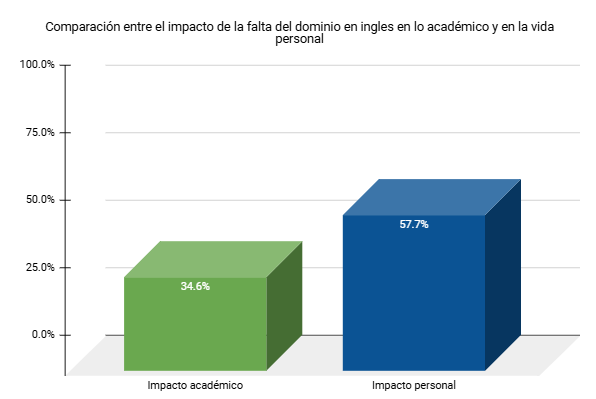
\includegraphics[width=0.8\linewidth]{Imagenes/Grafico impacto academico vs personal.png}
  \caption{Gráfico impacto académico vs personal}
  \label{fig:impactap}
\end{figure}

A partir de la \autoref{fig:impactap} podemos ver que el impacto de la falta de dominio del inglés es más significativo en la vida personal, con un 57.7\%, en comparación con el ámbito académico, que presenta un 34.6\%. Esto indica que las habilidades en inglés influyen mayoritariamente en situaciones personales y cotidianas que en el rendimiento académico. Sin embargo, no hay que ignorar el impacto académico, ya que también es significativo y afecta a una proporción considerable de la población.

\begin{figure}[H]
  \centering
  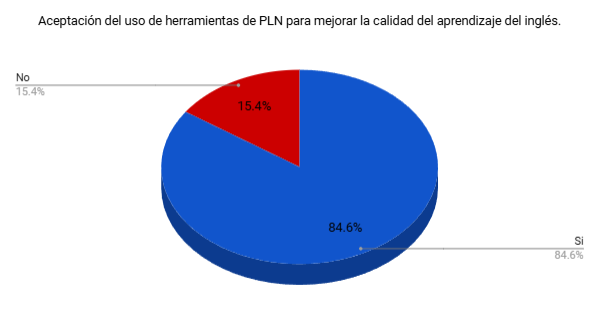
\includegraphics[width=0.8\linewidth]{Imagenes/Grafico 2 aceptacion del pln.png}
  \caption{Gráfico aceptación de herramientas de PLN}
  \label{fig:aceptpln}
\end{figure}


En la \autoref{fig:aceptpln} se puede evidenciar una alta aceptación del uso de herramientas de PLN para mejorar la calidad del aprendizaje del inglés, con un 84.6\% de personas a favor. Aunque una minoría del 15.4\% no está de acuerdo, la amplia mayoría sugiere un reconocimiento significativo del valor que estas herramientas pueden aportar en el proceso educativo.
\newpage
\begin{figure}[H]
  \centering
  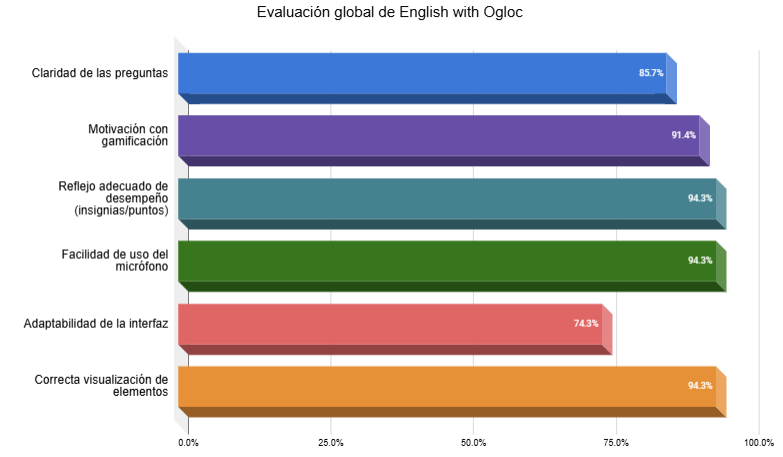
\includegraphics[width=0.9\linewidth]{Imagenes/Grafico 3 barras aceptacion general del prototipo.png}
  \caption{Gráfico evaluación global del prototipo}
  \label{fig:evalprot}
\end{figure}

En la \autoref{fig:evalprot} muestra una evaluación positiva del prototipo web en varias áreas clave, con alta satisfacción en el reflejo adecuado del desempeño y la correcta visualización de elementos (ambos con 94.3\%). La motivación con gamificación también es bien valorada, con un 91.4\%. Aunque la adaptabilidad de la interfaz tiene la valoración más baja con un 74.3\%, sigue siendo aprobada por la mayoría, indicando un desempeño sólido en general.


%%%%%%%%%%%%%%%%%%%%%%%%%%%%%%% Capitulo 8 %%%%%%%%%%%%%%%%%%%%%%%%%%%%%%%

\chapter{Conclusiones y trabajos futuros}
\section{Conclusiones}

De acuerdo con los resultados obtenidos en las encuestas y la síntesis general de la  \autoref{sintesis}, se puede concluir que una estrategia efectiva para mejorar la comprensión oral del inglés en la población bilingüe de Colombia es la integración de herramientas tecnológicas innovadoras que combinen metodologías interactivas y motivadoras con el uso de inteligencia artificial.
\\
\\
Los resultados de las encuestas revelan que los participantes consideran que el desconocimiento del inglés ha obstaculizado su rendimiento académico y sus oportunidades personales. Además, se reconoce el potencial del Procesamiento de Lenguaje Natural (PLN) como catalizador en el proceso de enseñanza-aprendizaje, destacando su capacidad para personalizar la experiencia y mejorar la calidad educativa.
\\
\\
En este contexto, el prototipo web English with Ogloc demostró ser funcional y atractivo para los usuarios. La facilidad de acceso a las lecciones, la claridad de los contenidos generados, y el uso del micrófono como herramienta para practicar la producción oral, son indicios de que un aplicativo web con enfoque en comprensión y producción oral puede ser una solución efectiva. Además, se presentó en el IV Encuentro Regional de Tesistas, donde también tuvo una aceptación positiva por parte del público y de los evaluadores. Adicionalmente, la incorporación de elementos de gamificación contribuyeron a elevar los niveles de motivación y compromiso.
\\
\\
Por tanto, para dar respuesta a la problemática de cómo mejorar la comprensión oral del inglés en Colombia, se recomienda fortalecer el desarrollo e implementación de plataformas que integren tecnologías emergentes, diseños centrados en el usuario y metodologías activas. Esta aproximación permite no solo facilitar la exposición al inglés hablado en contextos diversos, sino también impulsar una práctica constante que refleje el esfuerzo del usuario mediante retroalimentación y recompensas simbólicas. Todo ello apunta a cerrar las brechas existentes y potenciar las competencias comunicativas en inglés dentro de la población bilingüe colombiana.

\newpage
\section{Trabajos futuros}

Durante el desarrollo del prototipo se lograron identificar diferentes aspectos que complementarían y ayudarían al prototipo web a tener una mejora significativa:

\begin{itemize}
    \item Implementar un servicio para la funcionalidad de speech-to-text del prototipo. utilizar la librería gratuita Speech Web API lleva consigo a limitar el uso del prototipo a solo 2 navegadores en dispositivos de escritorio, lo cual al utilizar un servicio en la nube (de paga) esta limitación desaparecería, ademas que la calidad de la transcripción tendría una mejora significativa.

    \item Realizar el despliegue del prototipo en un servidor con GPU y una mayor cantidad de memoria RAM, para obtener un menor tiempo de generación de las lecciones, pues los modelos al ser procesados mediante GPU procesan a una mayor velocidad, y al tener mas memoria disponible, mejoraría la concurrencia en Celery.

    \item Realizar un ajuste fino a los modelos implementados con el objetivo de mejorar la generación, y la diversidad de las preguntas, llegando a poder realizar distintos tipos de preguntas o diversificando aun mas el contenido de las lecciones.
    
\end{itemize}

%%%%%%%%%%%%%%%%%%%%%%%%%%%%%%% Referencias %%%%%%%%%%%%%%%%%%%%%%%%%%%

\bibliographystyle{IEEEtran}            % estilo IEEE
\nocite{*}
\bibliography{Bibliografia}           % sin extensión .bib

%%%%%%%%%%%%%%%%%%%%%%%%%%%%%%% Anexos %%%%%%%%%%%%%%%%%%%%%%%%%%%

\newpage
\phantomsection
\label{Anexos}
\addcontentsline{toc}{chapter}{Anexos}
\chapter*{Anexos}

Los anexos los podrá encontrar en siguiente repositorio:
\begin{itemize}
    \item \url{https://github.com/BitzKort/Trabajo-de-Grado-Backend}
\end{itemize}

\section*{Historias de usuario}
\addcontentsline{toc}{section}{Historias de usuario}

Las historias de usuario se encuentran en la carpeta anexos bajo el nombre:

\begin{itemize}
    \item \texttt{Historias de Usuario Prototipo Web.pdf}
\end{itemize}

\section*{Encuestas}
\addcontentsline{toc}{section}{Encuestas}
Las 4 encuestas realizadas al prototipo y su usabilidad se encuentran en la carpeta anexos bajo el nombre:

\begin{itemize}
    \item \texttt{Encuesta de usabilidad basada en las Heurísticas de Jakob Nielsen.pdf}
    \item \texttt{Encuesta sobre niveles de ingles English with Ogloc.pdf}
    \item \texttt{Impacto de la Falta de Dominio del Inglés en tu Vida Académica y Profesional.pdf}
    \item \texttt{Prueba de usabilidad English with Ogloc.pdf}
\end{itemize}


\section*{Mockups y diseño responsive de la Interfaz de Usuario}
\addcontentsline{toc}{section}{Mockups y diseño responsive de la Interfaz de Usuario}

Todas las mockups de la Interfaz de Usuario y sus diseños responsive se encuentran en la carpeta anexos bajo el nombre:

\begin{itemize}
    \item \texttt{Mockups UI y diseño final Prototipo Web.pdf}
\end{itemize}

\section*{Documentos de participación en el IV Encuentro Regional de Tesistas}
\addcontentsline{toc}{section}{Documentos de participación en el IV Encuentro Regional de Tesistas}

El certificado de participación se podrá encontrar en la carpeta de anexos bajo el nombre:

\begin{itemize}
    \item \texttt{Certificado IV Encuentro Regional de Tesistas - Miguel Angel Rivera Reyes.pdf}
\end{itemize}

\end{document}
